\documentclass[12pt]{article}

\usepackage{wrapfig,color,multicol}
\usepackage{fancyhdr}
\usepackage{csquotes}
\usepackage{graphicx}
\usepackage{listings}
\usepackage{amsmath}
\usepackage{etoolbox}
\usepackage{color}

\numberwithin{figure}{section}
\numberwithin{equation}{section}

\AtBeginEnvironment{figure}{\stepcounter{equation}}
\AtBeginEnvironment{equation}{\stepcounter{figure}}

\usepackage[nottoc]{tocbibind}
\graphicspath{ {figures/} }
\usepackage[left=25.4 mm,right=25.4 mm,top=25.4mm]{geometry}


\usepackage[utf8]{inputenc}
\usepackage{t1enc}
\usepackage[magyar]{babel}
\linespread{1.5}
\usepackage{pdfpages}

\usepackage{footnote}
\usepackage{subfigure}
\usepackage{float}
\usepackage[]{algorithm2e}

\usepackage{xcolor}
\usepackage{hyperref}
\hypersetup{
	colorlinks,
	linkcolor=black,
	citecolor=black,
	urlcolor={blue!80!black}
}

\usepackage{listings}
\usepackage{xcolor}

\definecolor{codegreen}{rgb}{0,0.6,0}
\definecolor{codegray}{rgb}{0.5,0.5,0.5}
\definecolor{codegreen}{rgb}{0,128,0}
\definecolor{backcolour}{rgb}{0.95,0.95,0.92}
\definecolor{dkgreen}{rgb}{0,0.6,0}
\definecolor{gray}{rgb}{0.5,0.5,0.5}
\definecolor{mauve}{rgb}{0.58,0,0.82}
\definecolor{light-gray}{gray}{0.25}

\lstdefinestyle{Java}{
	backgroundcolor=\color{backcolour},   
	commentstyle=\color{codegreen},
	keywordstyle=\color{orange},
	numberstyle=\tiny\color{codegray},
	stringstyle=\color{codegreen},
	basicstyle=\fontsize{8}{9}\ttfamily,
	breakatwhitespace=false,         
	breaklines=true,                 
	captionpos=b,                    
	keepspaces=true,                 
	numbers=left,                    
	numbersep=5pt,                  
	showspaces=false,                
	showstringspaces=false,
	showtabs=false,                  
	tabsize=1,
	sensitive=true
}


\lstset{style=Java}



\begin{document}
	
\includepdf[pages={-},scale=1]{Borito.pdf}

\newpage

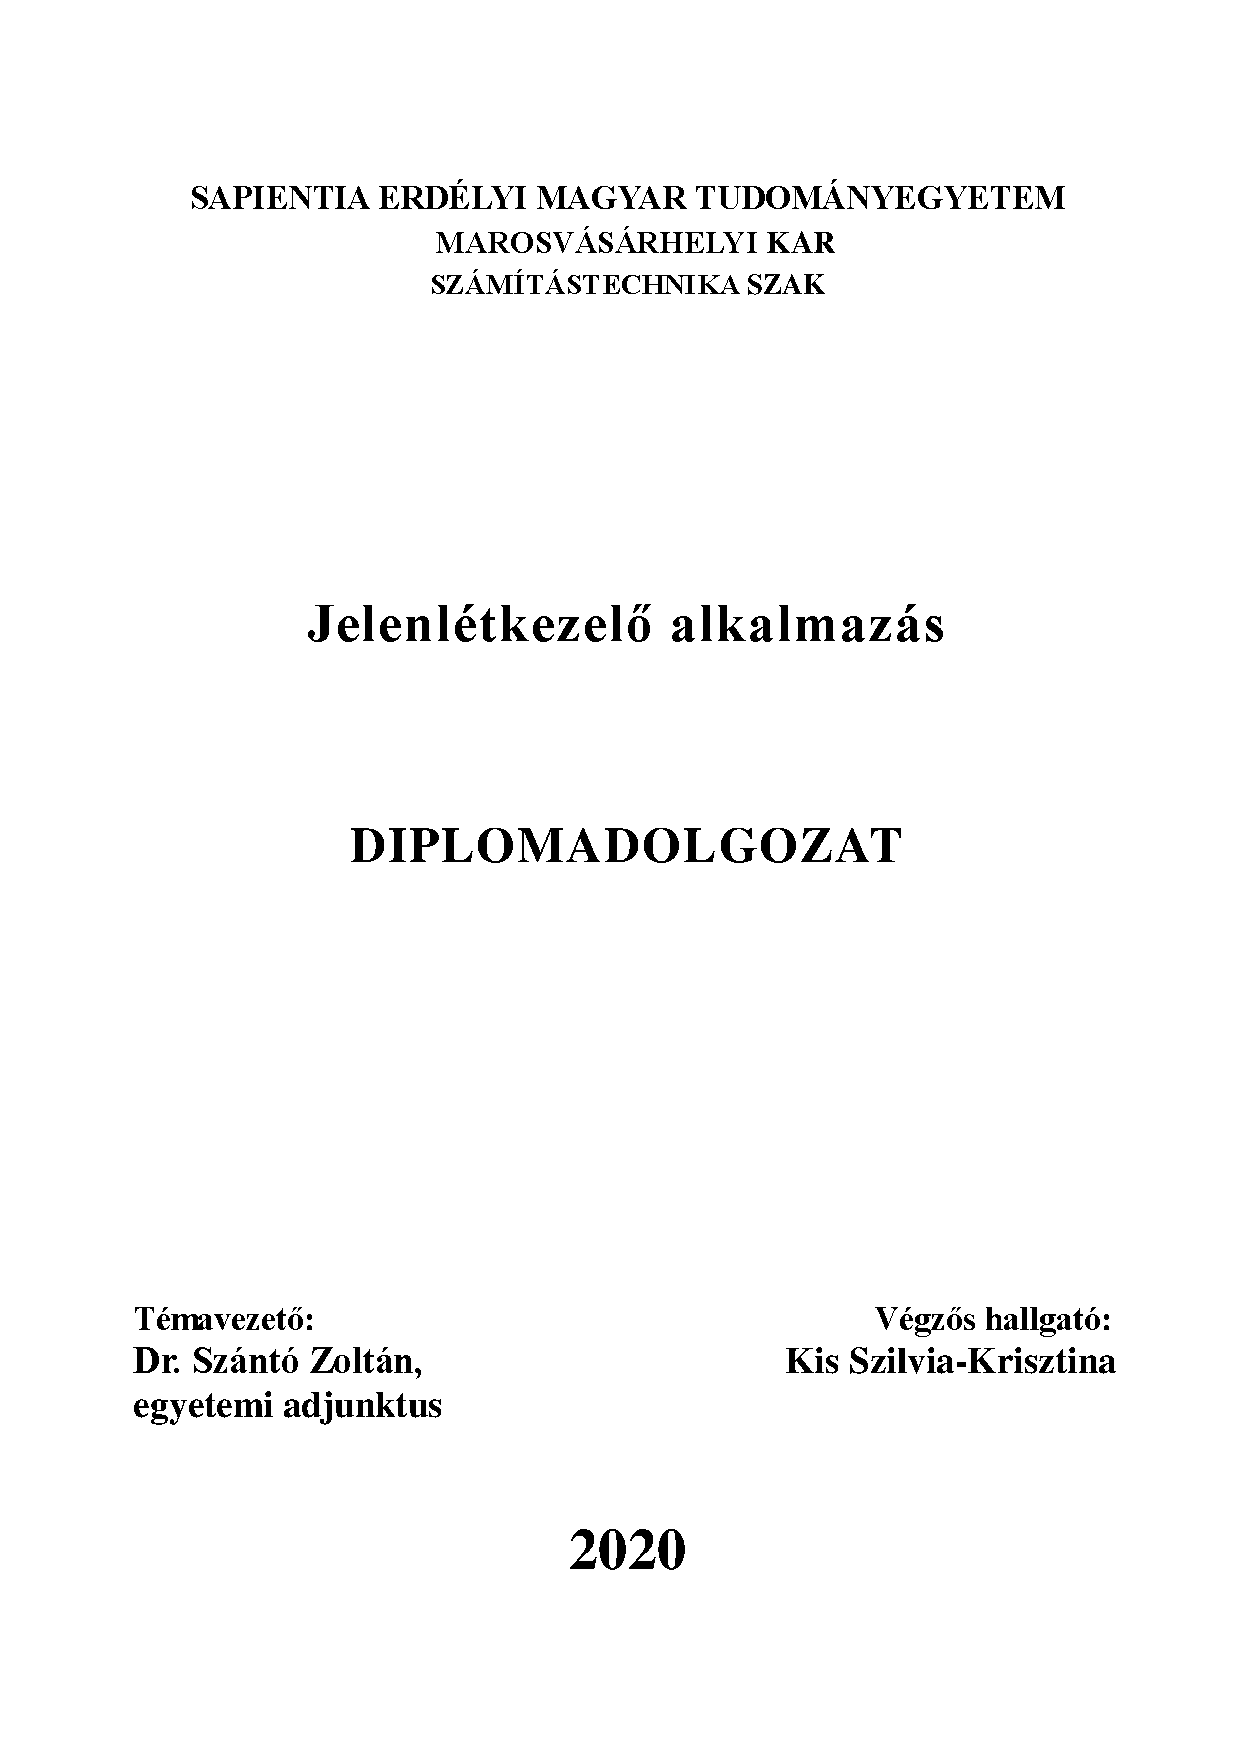
\includepdf[pages={-},scale=1]{ElsoLap2020.pdf}

\newpage


\includepdf[pages={-},scale=1]{MasodikLap2020.pdf}

\newpage

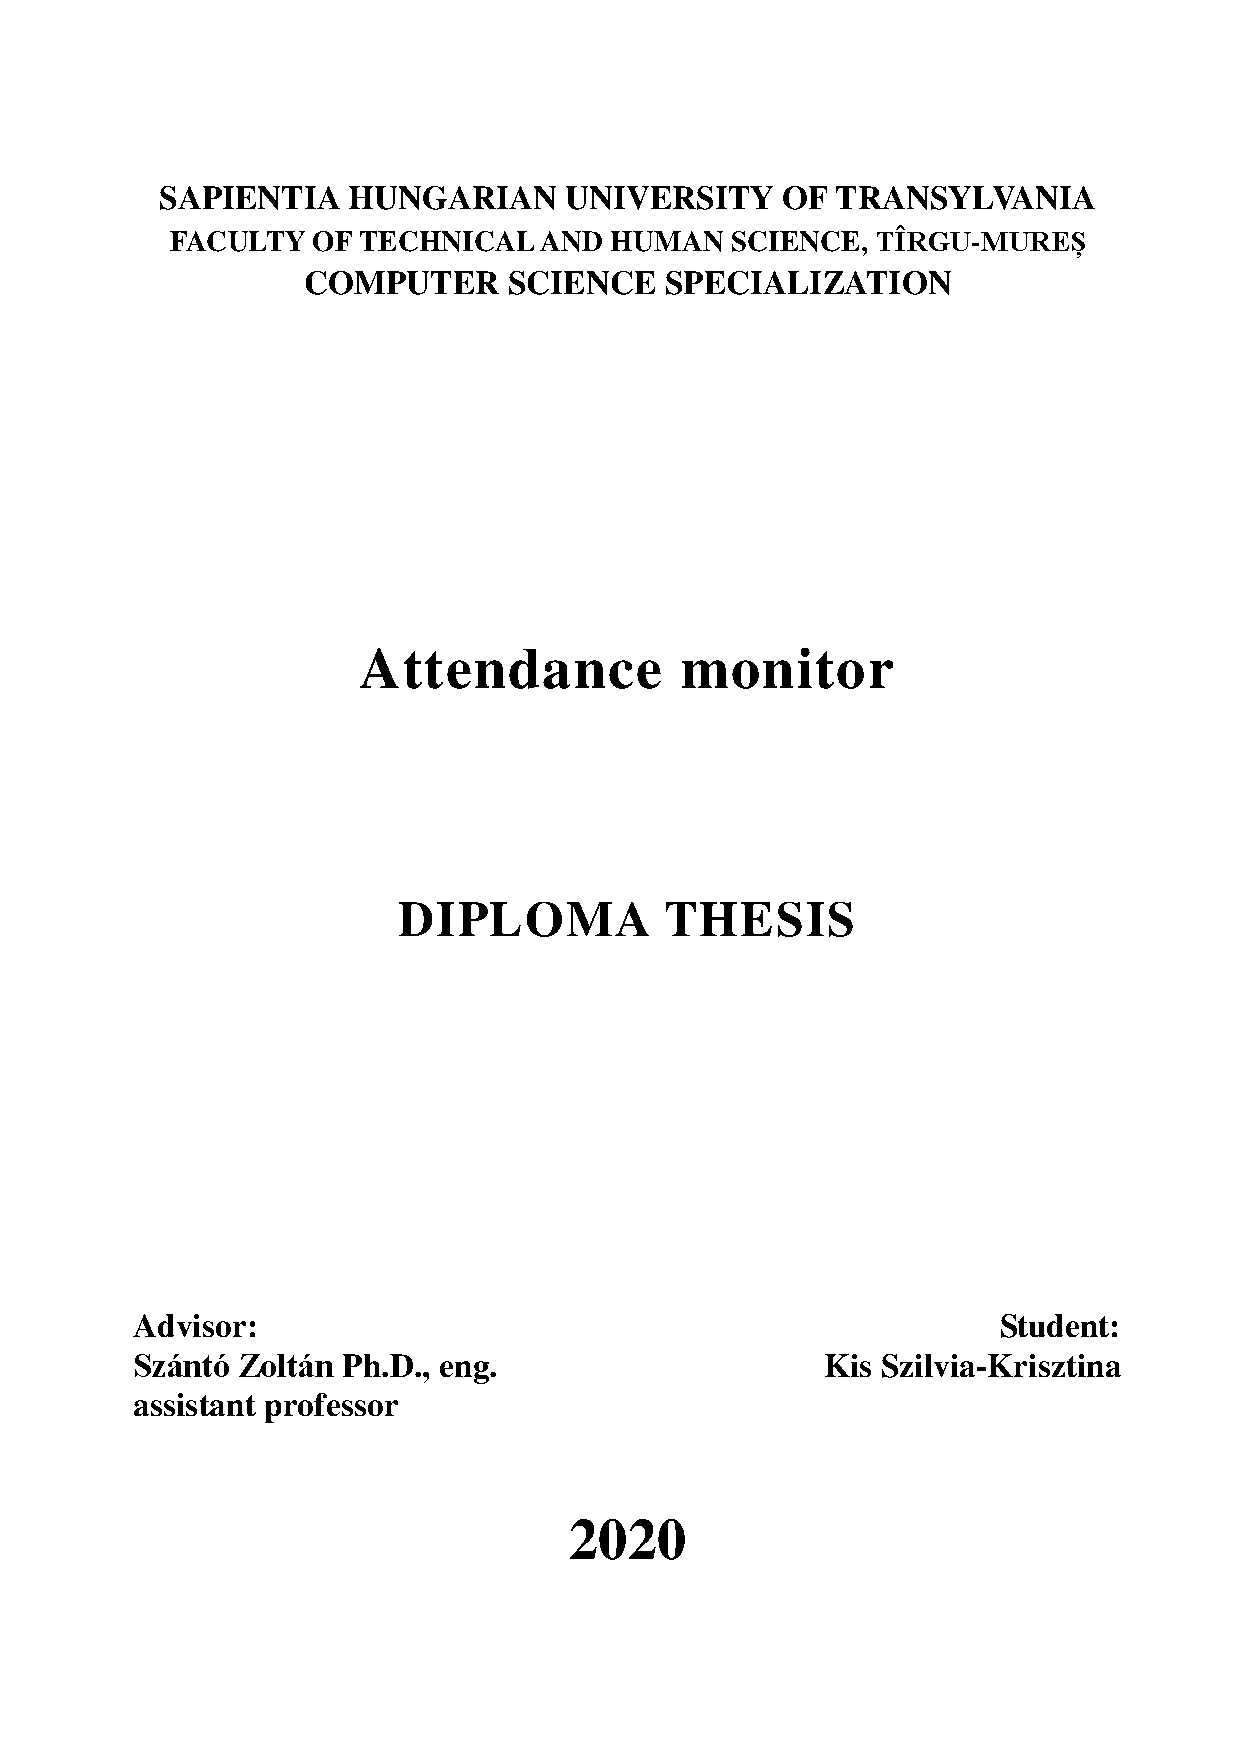
\includepdf[pages={-},scale=1]{HarmadikLap2020.pdf}

\newpage

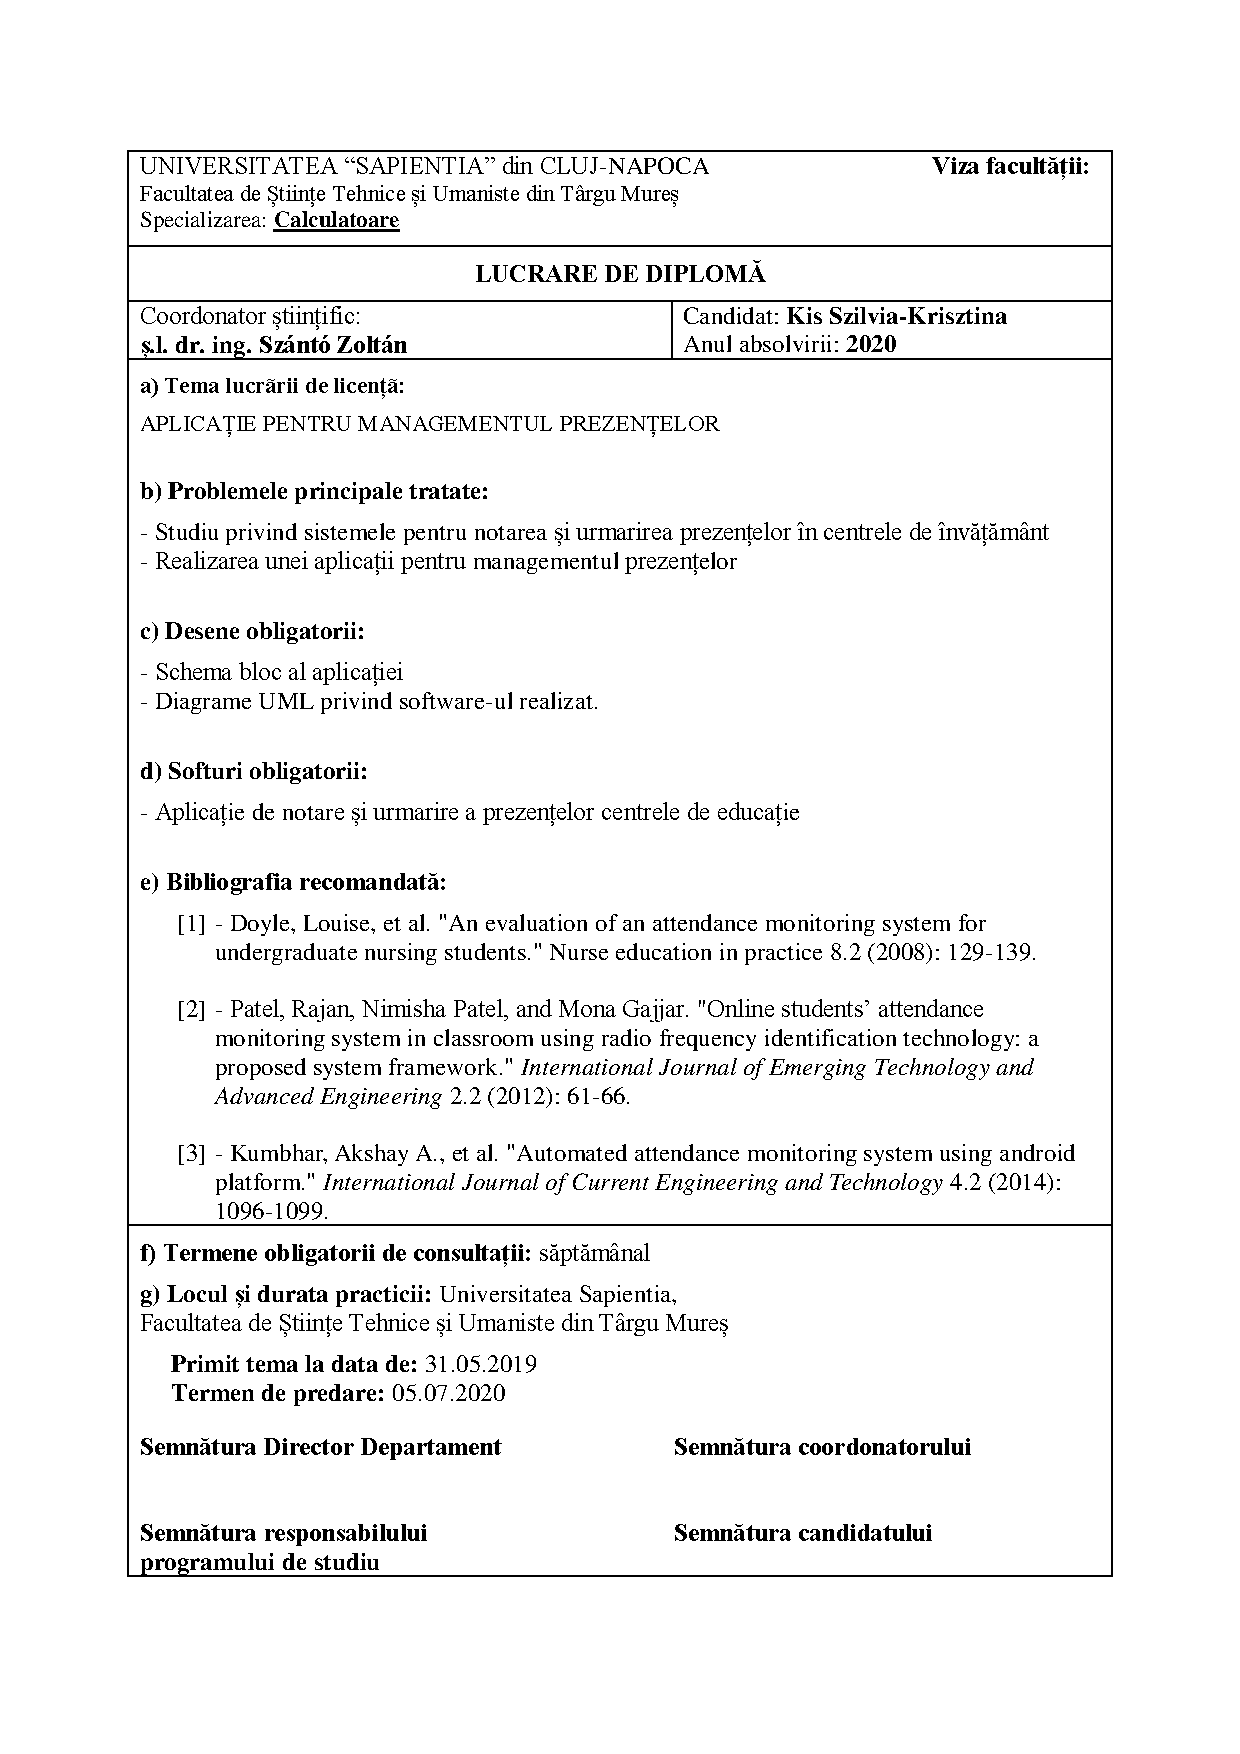
\includepdf[pages={1},scale=1]{tablazat.pdf}

\newpage

\includepdf[pages={-},scale=1]{declaratie.pdf}

\newpage

\thispagestyle{empty}
\section*{Kivonat}

A felsőoktatási intézmények nagy része még mindig a hagyományos eszközöket használja az órák során a hallgatók jelenlétének kezelésére. Ezek a módszerek általában nem hatékonyak, mivel egyenként be kell vezetni minden diákot, valamint nem kapunk egy pontos értéket arról, hogy egy diák mennyi időt volt az órán. Ugyanakkor ezen módszerek hátrány az is, hogy a késő diákok megzavarják az órát. \\
A dolgozat célja egy olyan szoftverrendszer megvalósítása, amely megkönnyíti az órákon való jelenlétkezelést, megbízhatóvá és hatékonyabbá téve azt, úgy a tanárok, mint a diákok számára, kihasználva az adott technológiai eszközöket.\\
A fejlesztett rendszer lehetővé teszi, hogy a diák saját okostelefonja segítségével jelentkezzen az adott órára, illetve lehetőséget ad a tanárnak, hogy a jelentkezéseket könnyedén kezelje. \\
Ebből kifolyólag a dolgozat két alkalmazást foglal magába: egy Diák, illetve egy Tanár applikációt, mivel mindkét félnek saját szerepköre van. A Diák alkalmazás létrehoz egy egyedi azonosítót, amely segítségével a Tanár alkalmazás azonosítja a diákot, így igazolva az órai jelenlétét. Ugyanakkor a rendszer minden azonosítást egy adatbázisba ment, amelyből kimutatásokat tud generálni.\\
Mindemellett a rendszer segíti a tanár-diák online kapcsolattartást és információ átadást, felkínálva a lehetőséget e-mail küldésre, naptár események létrehozására vagy akár Google tanterem alkalmazására.\\
A rendszer androidos telefonokra készült, QR kód segítségével történik az azonosítás, amely egyfajta titkosítást biztosít, illetve az adatok könnyebb elérése érdekében az adatbázis felhő alapú. \\
\\
\textbf{Kulcsszavak:} jelenlét, azonosítás, Android alkalmazás.

\newpage

\thispagestyle{empty}
\section*{Extras}

Majoritatea instituțiilor de învățământ superior utilizează în continuare instrumente tradiționale pentru managementul prezenței studenților în timpul lecțiilor. Aceste metode nu sunt eficiente, deoarece fiecare elev trebuie introdus unul câte unul, și nu primim o valoare exactă despre cât timp a fost un elev în clasă. Cu toate acestea, dezavantajul acestor metode este că elevii care ajung mai târziu la ore deranjează lecția.\\
Scopul acestei lucrări este de a implementa un sistem care facilitează managementul prezenței la cursuri, făcându-l fiabil și mai eficient pentru profesori și studenți, folosind instrumentele tehnologice disponibile.\\
Sistemul dezvoltat permite elevului să semnaleze prezența la curs folosind smartphone-ul său și permite profesorului să trateze cu ușurință.\\
Din acest motiv, teza include două aplicații: o aplicație Student și un Profesor, deoarece fiecare parte are propriul rol. Aplicația Student creează un identificator unic pe care aplicația Profesor îl utilizează pentru a identifica elevul pentru a-și nota prezența în clasă. Cu toate acestea, prezențele studenților sunt salvate într-o bază de date din care se pot genera rapoarte.\\
Sistemul este proiectat pentru telefoanele cu sistem de operare Android folosind codul QR, care oferă o formă de criptare, iar baza de date este bazată pe cloud pentru un acces mai ușor.\\
\\
\textbf{Cuvinte cheie:} prezența, identificare, aplicație Android.

\newpage

\thispagestyle{empty}
\section*{Abstract}
Most of schools, universities still use traditional methods for tracking the presence of its students during classes.These methods generally are not efficient, because every student has to be noted one by one, and we still didn’t get a good view of actual time a student spends in classes. The students who arrive later will disturbe the class, because their pressence must also be noted. This is another disadvantage of these older methods.\\
The goal of this work is to create a software system, which not just makes tracking and handling the presence easier, it is also more efficient and reliable for both sides, teachers and students, by using some technological devices from the day to day life.\\
The developed system allows the student to use his or her smartphone to apply for a given class, and also makes it easier for the teacher to handle these applies.
Based on the mentioned requirements this project includes two applications: one student application, and one teacher application for separating their roles. The student application creates a unique identifier which helps the teacher application to identify the student and to mark his attendance during class. All the attendances are saved in a centralized database which is also used for generating statistics based on their arrival time in class, and other criteria.\\
Apart from this, the system helps maintaining the teacher-student relation, information sharing between them by providing the possibility to send emails, create events and also to use the Google classroom.\\
The system targets smartphones with Android operating system, the identification of a students is done by generating and exchanging QR codes, which ensures a level of encryption, and all the data is saved in a cloud based database.\\
\\
\textbf{Keywords:} attendance, identification, Android application

\newpage

\thispagestyle{empty}
\tableofcontents
\thispagestyle{empty}

\newpage

\thispagestyle{empty}
\listoffigures
\thispagestyle{empty}
\newpage


\pagenumbering{arabic}
\section{Bevezető}

A mai ember nem tudja elképzelni az életét különböző digitális eszközök nélkül, köszönhetően a gyorsan fejlődő technikának, ami jelen van az életünk minden területén. Így van ez az oktatásban is. Napjainkban a digitális eszközök fontos szerepet játszanak az oktatásban, ezért fontos, hogy a tanügyi rendszer, valamint a tanárok is lépést tartsanak a rohamosan fejlődő világunkkal, bár ez nem mindig könnyű.\\
A felsőoktatási intézményekben tudnak legjobban viszonyulni az új technológiákhoz. Ez abban nyilvánul meg, hogy lehetőségeik szerint próbálnak minél korszerűbb módszereket használni az oktatás során. Azonban az egyetemek jó része még mindig a hagyományos eszközöket használja az adminisztratív tevékenységek elvégzésére. Ide tartozik a jelenlét kezelése is, ami egy gyakran ismétlődő procedúrát jelent, és amelyre többféle, kevésbé hatékony módszert használnak. Megemlíthetjük többek között a papír alapú jelenlétírást, amelynek több változatát is alkalmazzák. A legelterjedtebb amikor a diákok sorban felírják neveiket egy körbeadott papírra. Ez több szempontból is egy rossz módszer. Elsősorban könnyen kijátszható, mivel egy diák saját magán kívül bárki mást is felírhat, másrészt ez plusz munkával jár, mivel a tanárnak valamilyen szinten rendszereznie és nyilvántartania kell ezeket a jelenléteket. Hasonlóan ehhez a módszerhez, létezik egy olyan változat, amikor a tanár írja a névsort, körbekérdezve egyenként a diákokat. Ez minden bizonnyal az előzőtől is rosszabb módszer, mivel nagyon időigényes folyamat, és ez az idő az oktatásra szánt időből vonódik le. Másik gyakran használt módszer a névsorolvasás, ami feltételezi, hogy a tanár rendelkezik a diákok névsorával, azonban a hallgatók számától függően ez is sok időt elvesz az órából, így ez sem egy hatékony módszer.\\
Elmondhatjuk, a legfontosabb, hogy egy jól működő, megbízható és hatékony módszert alkalmazzunk az egyetemi órákon való jelenlét kezelésére.\\
A másik fontos szempont a kivitelezés. A legjobb módszer, ha egy olyan rendszert tudunk alkalmazni, ami csupán a mindenki számára adott technológiai erőforrásokat igényli, ilyen például a diákok okostelefonja, mivel bizonyára minden diák rendelkezik az eszközzel.\\
Több tanulmányban is olvashatunk arról, hogy hogyan vezetik be a különböző számítástechnikai eszközöket az osztálytermekbe. A legtöbb esetben különböző eszközöket is bevonnak, ilyen például az RFID. A hatékonyságot növeli, azonban erőforrás igénye miatt nem minden esetben kivitelezhető, ugyanakkor használata több újabb erőforrásokat vesz igénybe.
Létfontosságú, hogy az oktatási ágazatok olyan megoldásokkal rendelkezzenek, amelyek egyszerűsítik a jelenlét kezelését és növelik ezek hatékonyságát, mindazonáltal lehetőséget nyújtsanak mindenkinek ezek használatára.\\
A dolgozat során a tanórai jelenlétek kezelésének korszerűsítésére, illetve az ezzel járó problémák kiküszöbölésére kerestünk megoldásokat.\\
Fontos szempont, hogy a jelenlétkezlő alkalmazásnak minimális erőforrásigénye legyen, idő szempontjából hatékony, valamint minden szempontból megbízható, mivel néha sok múlhat egy-egy észre nem vett hibán. Felhasználás szempontjából fontos, hogy kerüljük a különböző engedélyszükséges adatok használatát, illetve amennyiben lehetséges, ne vegyünk igénybe más olyan alkalmazásokat amelyek jogosultság engedélyezésének szükségességét vonják maguk után. \\ 
A hagyományos módszerek többek között magukban hordozzák azt a hátrányt, hogy a diák számára nem követhetőek a jelenlétek, ami azt jelenti, hogy legtöbb esetben a diák nem tudja megtekinteni saját jelenléteit, pótlásait, vagy ami szintén nagyon fontos, a hiányzásait, mivel ezt a legtöbb alkalmazott módszer nem teszi lehetővé. A jelenlétkezelő rendszer szempontjából ez egy elvárt funkcionalitás kell legyen, mind a tanár, mind a diák számára. Mindemellett megemlíthetünk olyan előnyöket a modern jelenlétkezelő alkalmazás használata következtében, mint a statisztikák készítése a diák effektív órán töltött idejéről. Ezalatt azt értjük, hogy az alkalmazott rendszer a pontos időt tárolja amikor a diák megérkezik és bejelentkezik az órára, ezáltal kimutathatóvá válik, hogy az órák esetében általában mennyit késnek a diákok.\\
Az említett érvek csupán töredékei azoknak a számos előnyöknek, amit egy hatékony jelenlétkezelő rendszer nyújthat a hagyományos módszerekkel szemben.\\
Elmondhatjuk, hogy az oktatási rendszer korszerűsítésében elengedhetetlenek a hasonló újítások. A gyors, hatékony és megbízható jelenlétkezelés csak egy része az eredményes oktatásnak, ehhez szeretnénk hozzájárulni az általunk fejlesztett alkalmazással.

\newpage

\section{Szakirodalmi tanulmány}
A különböző szakirodalmi cikkek között keresgélve, a dolgozat témájával kapcsolatos kulcsszavakra, mint például \enquote{attendance monitor}, \enquote{attendance management system} a keresési eredmények igen számottevőek, mivel sok hasonló témájú projekt került már megvalósításra. Számos kidolgozott rendszer létezik már, amelyek különböző módszerek, technológiák révén valósítják meg a korszerű egyetemi jelenlétkezelést.

\subsection{RFID}
Az \cite{1} tanulmányban egy olyan megközelítésről olvashatunk, ami RFID-t  (Rádiófrekvencia-azonosítás) használ a diákok jelenlétének azonosítására. Az RFID lehetővé teszi az egyetem számára, hogy alkalmazkodjon az ilyen új technológiákhoz az egyetem jelenlétkezelő rendszerének javítása érdekében, figyelembe véve az olyan tényezőket, mint a megbízhatóság, az időmegtakarítás és az egyszerű ellenőrzés \cite{3}.  \\
Az RFID technológia fő előnye az automatizált azonosítás és adatgyűjtés, célja a már használt rendszerek, például vonalkódok költségeinek csökkentése. Bár az RFID technológiát sok évvel ezelőtt fedezték fel, csak az elmúlt évtizedben kezdték továbbfejleszteni, mivel a megvalósítás legfőbb korlátja a költség volt \cite{2}. \\
A tipikus RFID rendszerek négy fontos összetevőből állnak: RFID olvasó (RFID Reader), RFID címke (RFID tag), RFID köztes szoftver (RFID Middleware), adatbázis (Database Storage).\\
A lekérdezőnek is nevezett olvasó rádiófrekvenciás adatokat küld és fogad az antennákon keresztül a címkékből. Az olvasónak több antennája lehet, amelyek felelősek a rádióhullámok küldéséért és vételéért. A címke az adatokat tároló mikrochipből, egy antennából és egy hordozóból áll, amelybe a chip és az antenna fel van szerelve.\\
A köztes szoftver az a réteg, amelyen a nyers RFID-értékeket megtisztítják és kiszűrik, hogy az adatok alkalmazás-barátabbak legyenek. A beérkezett információkat az olvasóktól kapja, majd bizonyos technikákat alkalmaz, hogy a fogadott adatfolyamból csak a hasznos adatokat gyűjtse be. A szűrt rekordok, beleértve a címkét és az olvasó azonosítóit, valamint a leolvasott időbélyegzőjét, továbbítódnak az adatbázisba \cite{1}.  \\
Ez alapján működik a jelenlétkezelés is az RFID-t használó rendszerek esetében. Minden felhasználó rendelkezik egy eszközzel, melynek segítségével tudjuk azonosítani őket. Az adat szűrés után bekerül az adatbázisba, ahonnan lekérdezés során, különböző szűrőket használva megjeleníthető lesz a kívánt felületen.\\
Az említett tanulmányban vázolt jelenlétkezelő módszer minden bizonnyal hatékony és működőképes megoldás. Vannak azonban hátrányai is, ezért esetünkben ez nem volt alkalmazható. Hátrányai közül megemlítjük első sorban azt, hogy az RFID-t használó jelenlétkezelő rendszerhez szükség van különböző hardver eszközökre, amelyek költségigényesek, mindemellett amennyiben az olvasó rögzítve van, a teljes rendszer bár működőképes, de helyhez kötött. Ha egyetemi szinten, minden órán használni szeretnénk az RFID-s jelenlétkezelő rendszert, az azt feltételezi, hogy minden terem fel van szerelve a szükséges eszközökkel, ugyanúgy a diákok esetében is, minden diáknak rendelkeznie kell a használt eszközzel.\\
Amennyiben van lehetőségünk a fent említett hátrányok kiküszöbölésére, a rendszer hatékonyan alkalmazható. \\

\subsection{Biometrikus azonosítás}
A biometrikus azonosítás alapja, hogy a rendszer az ember valamilyen egyedi sajátosságáról (például ujjlenyomat, retina, hang, stb.) vesz mintát, azt átalakítja digitális adattá és eltárolja az adatbázisban. Amikor lesz aktuálisan levett minta (azaz belépés történik), ezt összehasonlítja az adatbázisban tárolt mintákkal. A hivatalos meghatározás szerint: \enquote{a biometria az alapján azonosít, ami az ember maga, nem pedig az alapján, amit tud (kód, jelszó), vagy amije van (kártya, távirányító)} \cite{5}.  \\

\subsubsection{Ujjlenyomat}
A \cite{4} tanulmányban egy olyan megvalósításról olvashatunk, amely biometrikus adatot használ fel a diákok azonosítására az osztálytermekben. \\
A dolgozatban használt biometrikus azonosítót az ujjlenyomat képezi. A megvalósított rendszer tanári beavatkozás nélkül működik, illetve az ujjlenyomat olvasó egy hordozható eszköz formájában került megvalósításra, így a diákok óra közben is tudják jelezni jelenlétüket. A jelentkezés csupán annyiból áll, hogy a hallgató az érzékelő felületre helyezi az ujját. Ez az eszköz begyűjti az ujjlenyomatokat és USB interfész segítségével tud kommunikálni a számítógéppel. Maga a hordozható olvasó akkumulátorral üzemeltethető. A tanár számára biztosítva van egy felhasználói felület, ahol menedzselni tudja az eszközt és a jelenléteket. \\
A ujjlenyomat olvasó modul a rendszer fő alkotóeleme. A mikrovezérlő irányítja az egész rendszert, amely az ujjlenyomat-modulból, a Real Time Clock-ból (RTC), a gombokból és a grafikus folyadékkristályos kijelzőből (GLCD) áll. Az LCD kijelző megjeleníti a diák jelenléti állapotát (sikeres párosítás, nem sikeres, vagy már jelentkezett) \cite{4}.  \\
Az olvasó eszköz akár fél évig is tárolja az adatokat, csak akkor van szükség a számítógéphez való csatlakozásra, ha látni kívánják az összesített jelenlétet, illetve exportálni akarják azokat.
A kivitelezett rendszer hatékony jelenlétkezelést biztosít, sőt ellenben az RFID technológiát alkalmazó megoldással, az ujjlenyomat azonosítás nagyobb biztonságot nyújt. Ez azt jelenti, hogy egy diák csak saját jelenlétét tudja igazolni, ellenben ha egy eszköz szolgál az azonosításra, azt fel tudják használni egymás helyett, így a rendszer kevésbé megbízható és ellenőrizhető.\\
Amint az látható az ujjlenyomat azonosítást végző rendszer számos előnnyel rendelkezik. Ezek közül megemlíthetjük az időtakarékosságot, a teljes megbízhatóságot, illetve a hatékonysághoz hozzátartozik a gyorsaság és az, hogy a tanárnak nem kell beavatkoznia, ezáltal a jelenlétkezelés semmilyen szempontból nem zavarja meg az órát.\\
Arra, hogy miért nem ezt a módszer alkalmaztuk az általunk megvalósított rendszerben, a válasz egyszerű. A legtöbb biometrikus azonosítást végző módszerek különleges hardver eszközöket igénylenek, amelyek beszerzése anyagilag megterhelő lehet. Higiéniai szempontból a fizikai érintkezést igénylő eszközök nem kedvezőek, főleg olyan esetekben, ahol naponta több száz vagy ezer ember használja az eszközt \cite{6}.  
Mindemellett a különböző biometrikus adatok tárolására és vételezésére jogszabályok vonatkoznak, amelyeknek ha nem tesznek eleget büntetőjogi következményei lehetnek.\\
Összességében az ujjlenyomattal történő jelenlétkezelés hatékony módszer, feltételezve, hogy anyagilag nem megterhelő a hardver eszközök beszerzése, illetve ha minden óvintézkedést megtettünk annak érdekében, hogy a rendszer használata következtében jogilag senki ne sérüljön.\\

\subsubsection{Arcfelismerés}
A \cite{7} tanulmány szintén egy biometrikus azonosítást alkalmazó módszert mutat be, ahol egy arcfelismerő rendszerrel azonosítják a diákokat az egyetemi órák során. \\
Az arcfelismerő rendszer lényege, hogy képes azonosítani vagy ellenőrizni egy személyt digitális képből vagy akár videoforrásból.\\
Az azonosítás két lépkésben történik. Első lépésben az arc körvonalát kell megkeresni, és eltávolítani a hátteret. Ha ez megvan, a második lépés során, a beazonosított arcot összehasonlítja a már adatbázisban lévő adatokkal, mivel a rendszer alapját képezi az is, hogy előzőleg úgymond \enquote{mintát} kell venni az adott személytől, és ezt tárolni, hogy azonosítás során legyen mivel összevetni. Az összehasonlításra két matematikai transzformációkon és analízisen alapuló eljárást használnak. Az egyik ilyen módszer az arcról készült képet, mint különböző árnyalatú foltokat vizsgálja, a másik módszer pedig az arc különböző alkotóelemeit keresi meg, mint például az orr, szemek, száj, stb., és azok helyzetét, egymástól való távolságát vizsgálja \cite{6}.  \\
A említett tanulmányban szokványos arcfelismerő rendszer került megvalósításra. Első lépésben az arc detektálása után következik a felismerési folyamat. A felismerés úgy történik, hogy a vélt arcot kivágva, vagyis a hátteret eltávolítva, összehasonlítja az adatbázisban lévő adattal. Ezt a folyamatot az érdekeltségi kör kiválasztásának nevezzük. Így egyenként ellenőrizve a hallgatók arcát, azok jelenlétei jelzésre kerülnek a szerveren. \\
A rendszer összességében egy kamerából áll, amely rögzíti az osztálytermi képeket és elküldi azt a képjavító modulhoz. Javítás után a kép átkerül az arcdetektáló és felismerő modulhoz, majd ezután kerül jelzésre a jelenlét az adatbázisba. Itt az összes arc felismerésre kerül a bemeneti képről, és az algoritmus egyenként összehasonlítja őket az adatbázisban tárolt arcokkal. A rendszerhez csatolva van egy órarend modul, így az automatikusan megkapja a tárgyat, az osztályt, a dátumot és az időt. Ahogy a tanár megérkezik az osztályba csupán egy gombnyomással elindítja a jelenlét rögzítését, így szinte teljes külső beavatkozás nélkül történik a jelenlétkezelés, megbízhatóan, ezáltal nagyon sok időt és adminisztratív munkát spórolva. A jelenléteket egy szerveren tárolják, így bárki hozzáférhet, tanárok, diákok, vagy esetleg a szülők.\\
A kamera folyamatosan készíti a képeket, hogy detektálni, valamint felismerni tudja az összes diákot az osztályban. A téves detektálás elkerülése érdekében a bőr osztályozási technikáját alkalmazzák. Ezzel a technikával a detektálási folyamat hatékonyabb és pontosabb lesz, mivel először a bőrt osztályozzák, majd csak a bőr képpontjai maradnak meg, és a kép összes többi pixelét feketére állítják \cite{7}. \\
Amint az érzékelhető, az ujjlenyomatot használó módszert felülmúlja, és számos előnnyel maga mögött hagyja a vázolt arcfelismerő rendszer. Előnyei közé sorolható, hogy semmilyen fizikai kontaktust nem igényel a rendszer, így a ujjlenyomat azonosítással ellentétben teljesen higiénikus. Továbbá az arcfelismerő rendszer egyike azon módszereknek, amelyek előzőleg igénylik az adott személy adatainak tárolását, ez esetben az arcról készített képet, amivel hasonlítani tudja majd a detektálás után, ezért vélhetően a detektált személy előzőleg beleegyezett abba, hogy az arcképe tárolva legyen a rendszer által. Hatékonyságát növeli az is, hogy egyszerre több arcot is azonosít, anélkül, hogy a diák bármit kellene tegyen ennek érdekében, ugyanakkor ez a hátránya is lehet a rendszernek. Ha egy diák takarásba van végig az órán, és nem tudja a rendszer detektálni az arcát, a jelenléte nem lesz elmentve. 
Hátrányai ennek a rendszernek is meghatározóak, mivel anyagi vonzata jelentős, illetve különböző jogi és adatvédelmi kérdéseket vethet fel, ha az adat beolvasása akár távolról, az adott személy beleegyezése nélkül is megtörténhet. Emellett a rendszer nem elég robosztus, zavarhatják a fényviszonyok, és nem utolsó sorban \enquote{kijátszható} például egy fotóval \cite{8}.

\subsection{Következtetés}
A különböző megközelítéseket tanulmányozva, olyan következtetéseket vonhatunk le, ami segít egy olyan rendszert kivitelezni, hogy az magába hordozza a már létező módszerek előnyeit, és minimálisra csökkentse a felmerülő hátrányokat.\\
Összességében elmondhatjuk, hogy egy általános és jól működő jelenlétkezelő módszer alapjai a következők:
\begin{itemize}
	\item {Azonosítás: szükség van egy azonosítóra, ami legyen egyedi és nehezen kijátszható.}
	\item {Eszköz: az igénybe vett eszköz legyen mindenki számára elérhető és a lehető legköltségtakarékosabb.}
	\item {Adattárolás: a rendszer alapját képező adatok tárolása a legfontosabb, ezért fontos, hogy az adatbázis valós idejű legyen, mindig naprakész és elérhető.}
	\item {Gyorsaság:  rendszer fő funkcionalitása, felismerni és rögzíteni a diák jelenlétét, elfogadható időkorlátok között.}
	\item {Titkosított kommunikáció: személyes adatok biztonsága, amely az azonosítás során sem válik nyilvános információvá a felhasználók számára.}
\end{itemize}
A rendszer fő jellemzője a gyorsaság, egyszerűség és hatékonyság kell legyen. Ezeket szem előtt tartva, valamint a szükséges alapkövetelményeknek eleget téve megvalósítható egy konzisztens jelenlétkezelő alkalmazás.\\
Összegzésként elmondható, hogy egy hatékony rendszer kivitelezésekor mindig meg kell találni a megfelelő egyensúlyt a biztonság és a használhatóság között. Sok esetben szükség van áldozatokra, mint például esetünkben, igénybe vesszük a felhasználó telefonját, ezzel valamilyen szinten kockáztatva az adatvédelmet ahhoz, hogy a rendszer használható legyen.  A felhasználó bele kell egyezzen az alkalmazás telepítésébe, illetve az ehhez szükséges engedélyek megadásába (kamera, internet). A fejtörést csak az okozza, hogy mekkora lehet a feláldozhatóság mértéke ahhoz, hogy egy könnyen/gyorsan/ingyen használható alkalmazást fejlesszünk.\\


\section{Célkitűzések}
A dolgozat célja egy korszerű jelenlétkezelő rendszer kidolgozása, amely eleget tesz napjaink technológiai elvárásainak. Elsősorban egy olyan rendszer megvalósítására törekszünk, amellyel hatékonyabbá tehetjük az órai jelenlétkezeléseket a diákok és tanárok számára egyaránt. A hatékonyság fogalma alatt először is az időtakarékosságot, illetve a gyorsaságot értjük, mivel célunk, hogy az alkalmazás használatával a jelenlétkezelés az oktatás idejéből a lehető legkevesebbet vegyen el.\\
Fontos szempont, hogy a projekt kivitelezése során olyan erőforrásokat használjunk fel, amely mindenki számára elérhető, illetve használata ne igényeljen plusz anyagi kiadásokat. Ezeket szem előtt tartva döntöttünk úgy, hogy a legalkalmasabb erőforrás a rendszer kivitelezésére az okostelefon, mivel napjainkban többnyire minden diák rendelkezik az eszközzel.\\
Célunk emellett, nem csak a jelenlétek bevitele, hanem azok megtekintés, nyomonkövetése is, ami feltételezi, hogy a tanár minden diák esetében nem csak bevinni, hanem megnézni, valamint ha szükséges letölteni is tudja a jelenléteket, különböző szempontok szerint. Hasonlóan a diák esetében, aki a saját jelenléteit tudja követni, tantárgyakra lebontva.\\ 
Egy olyan funkcionalitás kivitelezése is szükséges, amely lehetővé teszi a tanár számára a jelenlétek exportálást. Ez azt jelenti, hogy az alkalmazásban a tanár számára lehetőség van a jelenléti táblázatok exportjára/letöltésére, ha szükséges több formátumban. A felhasználhatóság miatt az adott fájlt lokálisan menteni kell. 
A dolgozat célkitűzései között szerepel a statisztikák készítése is, ami a diák effektív órán töltött idejéről ad pontos értéket. Ezzel a funkcionalitással a tanár számára szeretnénk lehetőséget nyújtani, hogy nyomon tudja követni a diákok esetében mennyi időt töltenek az adott órán, mivel ismerjük az órák számának pontos értékét időben meghatározva, valamint a diákok érkezésének idejét is az alkalmazás által.\\
Bár a rendszer szerepkörét meghaladja, az online oktatás kihívásaiból inspirálódva, célunk lett egy olyan funkcionalitás bevezetése, amely egyszerűbbé teszi az online kurzusok elérését. Ez azt jelenti, hogy a jelenlétkezelő alkalmazásban minden tantárgyhoz rendelünk egy Google tantermet (Google Classroom), így amennyiben a tanár igénybe szeretné venni, csupán egy kattintással elérhető számára, és ugyanígy a diák esetében is. Emellett lehetőséget szeretnénk biztosítani az online kapcsolattartás leegyszerűsítésére is, melynek keretén belül szükségesnek látjuk az e-mail küldési lehetőséget mind a tanár, mind a diák részéről. A tanárnak lehetőséget adunk a szak valamint a tantárgy kiválasztása által a csoportos e-mail küldésre, illetve a diáknak, hogy egy tanárokat tartalmazó névlistából kiválasztva tudjon személyes üzenetet küldeni, anélkül, hogy ismernie kellene a tanár e-mail címét.\\
Elmondható, hogy ezen célkitűzések megvalósítása révén már egy hatékony jelenlétkezelő alkalmazást tudunk biztosítani a felhasználók számára, ugyanakkor még számos továbbfejlesztési lehetőségeink vannak a fent említett célok mellett.


\section{Szoftver követelmények}
\subsection{Felhasználói követelmények}

A rendszernek két típusú identifikált felhasználója van az egyetemen belül mégpedig a diákok és tanárok személyében. A felhasználói követelmények feltárása érdekében készítettünk egy használati eset (use case) diagramot, amely a ~\ref{fig:usecase} ábrán látható. A következőkben részletezve lesznek a különböző követelmények,szerepkörönkénti felosztásban.

\newpage

\begin{figure}[H]
	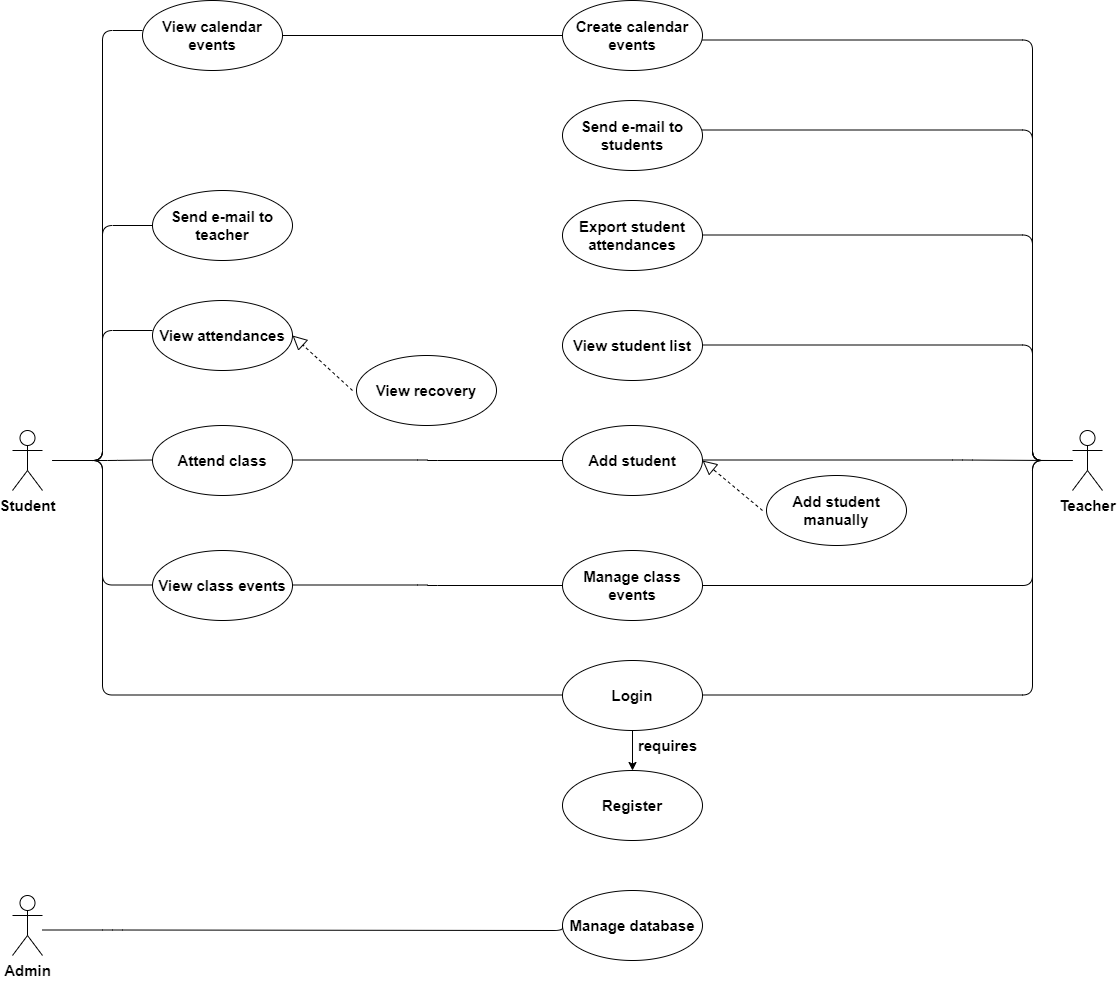
\includegraphics[width=\textwidth]{UseCase.png}
	\caption{A rendszer használati eset diagramja}
	\label{fig:usecase}
\end{figure}

\hfill\break

\subparagraph*{Diák}

\begin{itemize}
	\item {Regisztráció és bejelentkezés lehetősége, ezáltal lesz a diák a rendszer felhasználója.}
	\item {Jelentkezés az órára, ezzel a funkcionalitással a diák jelenlétét tudja igazolni az adott órán.}
	\item {Az órai jelenlétek, illetve pótlások számának, valamint azok időpontjának a megtekintése, aminek segítségével a diák követni tudja saját jelenléteit.}
	\item {E-mail küldése a tanárnak.}
	\item {Belépés a különböző tantágyak Google tantermeibe.}
	\item {Belépés a Neptun rendszerbe.}\\
\end{itemize}

\subparagraph*{Tanár}
\begin{itemize}
	\item {Regisztráció és bejelentkezés lehetősége, ezáltal lesz a tanár a rendszer felhasználója.}
	\item {A tantárgyi adatok megadása az új jelenlét beviteléhez.}
	\item {Diák hozzáadása a jelenléti listához.}
	\item {A korábbi jelenlétekkel rendelkező diáklista megtekintése, keresési lehetőség a diákok neve alapján, így nyújtva lehetőséget a tanár számára a diákok jelenléteinek követésére.}
	\item {Egy diákot kiválasztva annak részletes jelenlétei, pótlásai, illetve azok idejének megtekintése.}
	\item {Jelenlétek exportálása (letöltése), amely által a jelenléti ív mentésre kerül az eszközön későbbi megtekintésre vagy felhasználásra.}
	\item {Belépés a különböző tantágyak Google tantermeibe.}
	\item {Csoportos e-mail küldése a diákoknak.}
	\item {Naptáresemény létrehozása és elküldése a diákoknak.}\\
\end{itemize}

\subparagraph*{Adminisztrátor}

\begin{itemize}
	\item {Adatok karbantartása.}
	\item {Minden év elején feltölti a tantárgylistát, hozzárendeli a tanárokhoz a tantárgyakat, valamint a Google tantermet a tantárgyak esetén.}\\
\end{itemize}

\subsection{Rendszer követelmények}
\subsubsection{Funkcionális követelmények}
\subparagraph*{Diák}
\begin{itemize}
	\item {Regisztráció és adatok validálása: szak kiválasztása legördülő listából, teljes név, pontosan 6 karakter hosszúságú Neptun azonosító, e-mail cím, amely eleget tesz a formátumnak, minimum 6 karakter hosszúságú jelszó, majd ezek tárolása NoSql adatbázisban, a \enquote{Regisztráció} gomb lenyomásával.}
	\item {Bejelentkezés: azzal az e-mail és jelszó párossal, amely korábban tárolva lett az adatbázisban regisztráció által, mindez a \enquote{Bejelentkezés} gomb lenyomásával.}
	\item{Amennyiben nem emlékszik a regisztrált jelszóra, az erre utaló szövegre kattintva lehetőség van új jelszó beállítására, amit a regisztrált e-mail címre küldött linkkel tehet meg.}
	\item {E-mail cím visszaigazolása, megerősítése a regisztrált e-mailre kapott link alapján, illetve amennyiben nem érkezett meg az e-mail, a \enquote{Visszaigazoló e-mail újraküldése} gombbal megismételhető a procedúra.}
	\item {A regisztrációt, illetve a bejelentkezést követően a rendszer generál egy QR kódot, amely a következő adatokat kódolja: Neptun azonosító, eszköz azonosító, teljes név, szak.}
	\item {\enquote{Jelenlét megtekintése} gombra kattintva, kiválasztható a tantárgy és annak típusa legördülő listából}
	\item{Ezt követően a \enquote{Megjelenítés} gombra kattintva, láthatóvá válik a meglévő jelenlétek száma, és a részletes jelenléti adat egy listában, a jelenlét típusa szerint megkülönböztetve: a hét, a beviteli dátum, valamint a jelenlét típusa (jelenlét-zöld, pótlás-sárga).}
	\item {\enquote{Egyéb alkalmazások} lehetőséget választva a diák három lehetséges opcióból választhat: \enquote{E-mail küldése a tanárnak}, ami lehetővé teszi a tanárnak való üzenetküldést a tanár nevének kiválasztása alapján, az e-mail cím ismerete nélkül. \enquote{Belépés a Google tanterembe} és \enquote{Belépés a Neptunba} opciók az adott alkalmazások megnyitását biztosítják.}\\
\end{itemize}


\subparagraph*{Tanár}
\begin{itemize}
	\item {Regisztráció és adatok validálása: teljes név, pontosan 6 karakter hosszúságú Neptun azonosító, e-mail cím, amely eleget tesz a formátumnak, minimum 6 karakter hosszúságú jelszó, majd ezek tárolása NoSql adatbázisban, a \enquote{Regisztráció} gomb lenyomásával.}
	\item {Bejelentkezés: azzal az e-mail és Neptun azonosítóval, amely korábban tárolva lett az adatbázisban regisztráció által, mindez a \enquote{Bejelentkezés} gomb lenyomásával.}
	\item{Amennyiben nem emlékszik a regisztrált jelszóra, az erre utaló szövegre kattintva lehetőség van új jelszó beállítására, amit a regisztrált e-mail címre küldött linkkel tehet meg.}
	\item {\enquote{Új jelenlét hozzáadása} menüpontot kiválasztva lehetőség van a különböző tantárgyi adatok megadására a rendelkezésre álló legördülő listák segítségével.}
	\item {Az tantárgyra vonatkozó adatok megadása után, a \enquote{Tovább} gombra kattintva megjelölhető a pótlás egy jelölőnégyzet segítségével, valamint két lehetséges módja van a diák hozzáadására a jelenléti listához.}
	\item{Amennyiben a diák regisztrált az alkalmazásban és rendelkezik a generált QR kóddal, a\enquote{Scan indítása} gombal a tanár hozzáadhatja a jelenléti listához a QR kód szkennelésével, így a diák adatai bekerülnek az adatbázisba.}
	\item {Amennyiben a diák nem rendelkezik az azonosításhoz szükséges eszközzel, lehetőség van az adatok manuális bevitelére, amelyhez szükségeltetik a szak kiválasztása egy legördülő listából, diák nevének és Neptun azonosítójának megadása, valamint a jelölőnégyzet segítségével jelezhető a pótlási szándék.}
	\item {\enquote{Korábbi jelenlétek megtekintése}: szak, tantárgy és annak típusának kiválasztásával legördülő listából, a 
	\enquote{Diákok megjelenítése} gombra kattintva megjelenik a jelenléti lista a diákok neveivel, valamint egy keresősáv, amely lehetővé teszi a diákok neve alapján való keresést.}
	\item {Egy diákot kiválasztva további adatok megtekintésére van lehetőség a diák jelenléteivel kapcsolatban, amely által látható a diák neve, és jelenléti adatai egy listában: hét, dátum, jelenlét(zöld), pótlás(sárga).}
	\item {\enquote{Jelenlétek exportálása} menüpont lehetővé teszi tantárgy és formátum függvényében való letöltést, ahol a kívánt tantárgyat egy legördülő listából választható, valamint annak formátuma is.}
	\item {\enquote{Belépés a Google tanterembe}: kiválasztva a kívánt tantárgyat, az alkalmazáson keresztül megnyitható a kívánt tanterem linkje.}
	\item {\enquote{Naptáresemény létrehozása} opció lehetővé teszi adott tantárggyal kapcsolatos esemény létrehozását, majd kiküldését a kiválasztott Google tanterem diákjainak.}
	\item {Az \enquote{E-mail küldése} lehetőség a csoportos e-mail küldést jelenti a diákok felé, szak és tantárgy függvényben.}\\
\end{itemize}

\subparagraph*{Adminisztrátor}
\begin{itemize}
	\item{Hozzáférés az adatbázisban tárolt adatokhoz.}
	\item{A tanár tantárgyainak menedzselése: tantárgy hozzárendelése a tanárhoz az adatbázisban a már meglévő tantárgylistához.}
	\item{Google tanterem menedzselése: minden tantárgyhoz létrehoz egy tantermet, és ennek URL címét szintén tárolja az adatbázisban lévő erre a célra létrehozott listában.}\\
\end{itemize}


\subsubsection{Nem-funkcionális követelmények}

\begin{itemize}
	\item {Az alkalmazások futtatása Android operációs rendszert támogató eszközön lehetséges, mindkét alkalmazás esetében  minimum Android 4.1 Jelly Bean (16. API szint) szükséges.}
	\item {A diák és tanár regisztrált adatainak tárolása egy valós idejű adatbázisban történik, ehhez esetünkben Firebase szükséges.}
	\item{Az azonosítás szintén a Firebase nyújtotta funkcióval valósul meg.}
	\item {Az aktuális jelenlétek lekérdezéséhez, valamint a regisztráció során küldött e-mail visszaigazolásához szintén internetkapcsolat szükséges.}
	\item {A Google tanterembe való belépéshez az internetkapcsolat mellett egy aktív Google fiókra is szükség van.}
	\item {A diák azonosítójának szkeneléséhez a tanár alkalmazást használó eszköznek rendelkeznie kell kamerával, valamint engedélyezni kell az alkalmazás hozzáférését.}
	\item{A jelenlétek tárolását, bevitelét, valamint lekérését a használt adatbázis biztosítja.}
	\item{A jelenléti adatok xlsx, pdf vagy csv formátumban exportálhatóak, ez a Google Apps szkripten keresztül valósul meg.}
	\item{A fájlok letöltése után, amennyiben meg szeretnénk nyitni (azonban ez már nem a rendszer feladata) szükség van a megjelenítést lehetővé tévő alkalmazásra, például Excel, PDF.}
	\item{Az e-mail küldési lehetőséghez aktív e-mail fiókra van szükség, illetve egy e-mail küldő alkalmazás meglétére az adott eszközön.}
	\item{A naptáresemény létrehozásához, valamint megtekintéséhez egy Naptár alkalmazás szükségeltetik, a kiküldött események megtekintéséhez kifejezetten a Google naptár alkalmazásra van szükség.}
	\item {A Google tanterembe való belépéshez internetkapcsolat, illetve egy aktív Google fiókra van szükség.}\\
\end{itemize}


\section{A rendszer részletes leírása}
\subsection{Rendszer architektúra}

\begin{figure}[H]
	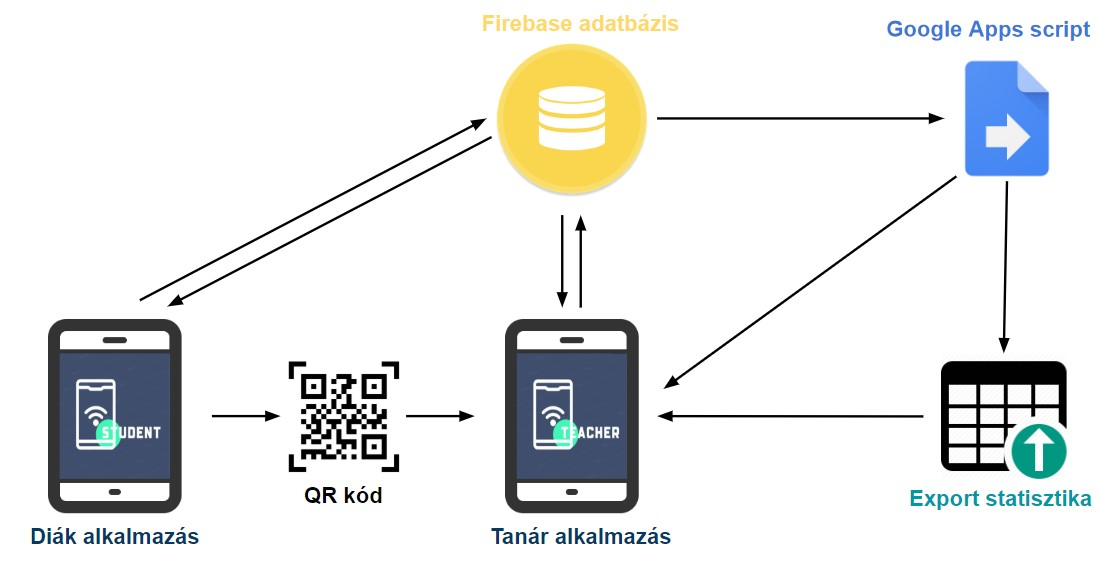
\includegraphics[width=\textwidth]{architecture2.jpg}
	\caption{A rendszer architektúrája}
\end{figure}

\hfill \break
Az alkalmazások egy közös Firebase adatbázissal rendelkeznek, amely tárolja a beérkező adatokat, valamint szolgáltatja azokat megjelenítésre. Tehát az alkalmazások kommunikációja az adatbázissal kétirányú.\\
A diák alkalmazás a QR kódon keresztül kommunikál a tanár alkalmazással, ezzel azonosítva magát.\\
A Google Apps script biztosítja az adatbázisból lekért adatok exportálását táblázatokba, ami letölthető a tanár alkalmazásban. Az alkalmazáson keresztül történik a szkript futtatása, amikor a felhasználó kívánja letölteni a jelenléti listát.\\

\hfill\break

\subsection{Titkosítás és átjátszhatóság}
Egy jelenlétkezelő alkalmazás esetében a legfontosabb kritériumot a biztonság és titkosítás kell jelentse, valamint fontos, hogy a rendszer ne legyen könnyen kijátszható. Ezalatt azt érjük, hogy a tárolt jelenlétek, valamint a felhasználók adatainak biztonságát a lehetőségeinkhez mérten fedezni kell.\\
A diák azonosítására szolgáló adatok QR kód formájában kerülnek titkosításra, amelyből csak a megfelelő alkalmazással és adatfeldolgozással kerülnek tárolásra.\\
A rendszer átjátszhatósága is fontos szempont, mivel a jelenlétek megbízható és valós értéket kell mutassanak. Az alkalmazásban erre külön ellenőrzéseket alkalmaztunk. Ide tartozik a diák által használt eszköz azonosítása, amely által egy eszközzel csak egy diák regisztrálhat. Ez az azonosító is kódolva lesz a QR kódban, így minden szkennelés esetén ellenőrizve lesz, hogy ugyan arról az eszközről történt a diák azonosítójának létrehozása vagy sem. Ezzel ki tudjuk szűrni, hogy egy diák több azonosítóval, azaz más diák helyett is jelentkezzen az adott órán. A nagyobb megbízhatóság érdekében bevezettünk emellett egy másik ellenőrzést is, ami a Neptun azonosítókat vizsgálja. Ez azt jelenti, hogy amikor a diák regisztrációkor megadja a saját Neptun azonosítóját, a rendszerben ellenőrizve lesz, hogy létezik-e már a megadott kód. Ezzel tesszük lehetővé egy alkalmazáson belül a több Neptun azonosítóval történő regisztráció kivédését.\\
Mindemellett a Firebase-ben történik a felhasználók hitelesítése, mivel az adatbázis nyújtotta autentikálást használjuk. Ezzel biztosítva van, hogy egy e-mail címmel csak egyszer lehet regisztrálni, valamint a jelszavak hash kódokká alakítva lesznek mentve, így senki számára nem lesz látható.\\

\subsubsection{Kiterjesztés}
A QR kóddal történő titkosítás olyan szempontból biztonságos, hogy emberi szem nem tudja értelmezni a benne lévő információt, azonban akár az újabb okostelefonok már dekódolni tudják csupán a kamera segítségével. Ez azért jelenthet gondot, mivel esetünkben személyes információk kerülnek kódolásra. Egyelőre ez nem jelent komolyabb veszélyt ami az alkalmazás használatát illeti, azonban erre is vannak már megbízhatóbb alternatívák, amelyekkel nem kell kockáztatnunk a személyes adataink biztonságát. Ilyen például a \cite{17} szemléltető által bemutatott random generált értékkel történő azonosítás. Ebben az esetben semmilyen személyes adat nem kerül a rendszerbe, csupán egy generált értékkel monitorizál embereket, így nem kell feláldozni a felhasználók privát adatait.\\
Bár a módszer esetén nem lesznek tárolva személyes adatok, azonban esetünkben ezen adatok megléte a rendszer pontos működéséhez járul hozzá, így nélkülözhetetlen az információk tárolása a felhasználóinkról. Annyival azonban hozzájárulunk az adatbázisban tárolt felhasználói információk biztonságához, hogy ezen adatokat tároljuk ugyan, de nem publikáljuk azokat, csupán a tanárnak áll jogában megtekinteni a diákok jelenléteit és az ehhez tartozó neveket és Neptun azonosítókat. Mivel ezek az információk az egyetemen belül is publikusak, nem követünk el személyi jogsértést. \\

\subsection{A rendszer osztálydiagramjai}

Az ~\ref{fig:class2} osztálydiagram vázolja a diák alkalmazás fő komponenseit és funkcionalitásait, amelyek közé tartozik a regisztráció és bejelentkezés, a rendszer általi QR kód generálás a diák azonosítására, valamint a korábbi jelenlétek listázása. Emellett látható az e-mail küldés modul is, valamint a Google tanterembe és Neptunba való belépés.\\

\begin{figure}[H]
	\centering
	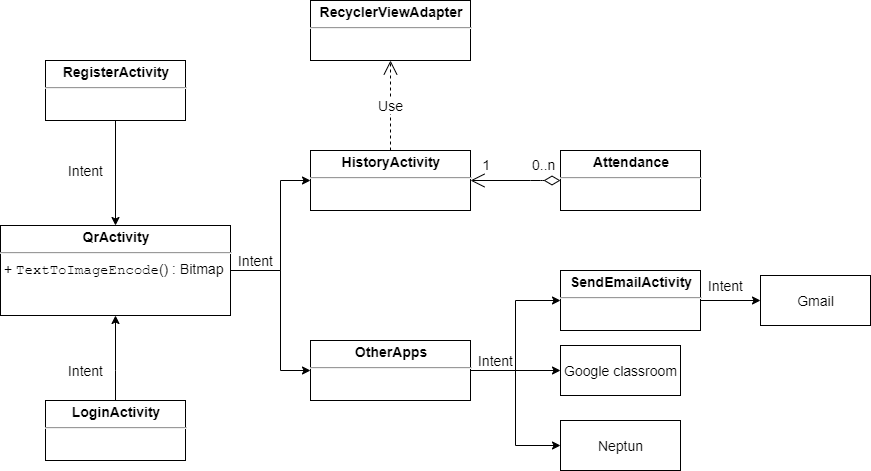
\includegraphics[width=400px]{stud_class.png}
	\caption{Diák alkalmazás osztálydiagramja}
	\label{fig:class2}
\end{figure}


\hfill\break
A tanár alkalmazás esetében (~\ref{fig:class1} ábra) is szerepel a regisztráció és bejelentkezés, amely fontos a tanár tantárgyainak beazonosítása végett.\\
Az alkalmazás fő komponensei a új jelenlét bevitele kétféle módon, a jelenétek listázása és letöltése, valamint a Google tanterembe való belépés, a naptár esemény létrehozása és az e-mail küldés.\\

\begin{figure}[H]
	\centering
	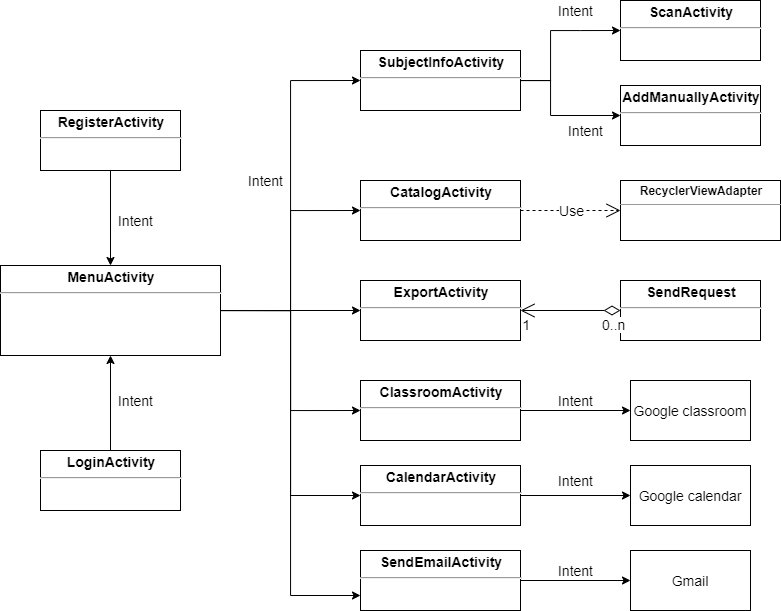
\includegraphics[width=400px]{teacher_class.png}
	\caption{Tanár alkalmazás osztálydiagramja}
	\label{fig:class1}
\end{figure}

\hfill\break

\subsection{A rendszer szekvencia diagramjai}

Az alábbi szekvencia diagramok a rendszer fontosabb moduljainak működését mutatják be.\\
Amint a ~\ref{fig:seq1} ábra szemlélteti, a tanár kiválasztja az adott tantárgyhoz tartozó adatokat, majd azok kitöltése után elindítja a szkennelést. Szkennelés során beolvassa a QR kódot, ezáltal menti a jelenlétet az adatbázisba. A mentést követően megjelenik a sikeres szkennelést jelző üzenet.\\

\begin{figure}[H]
	\centering
	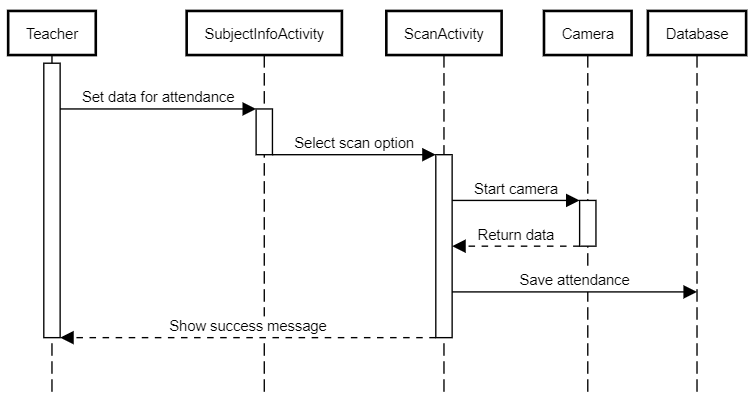
\includegraphics[width=350px]{seq_addScan1.png}
	\caption{Jelenlét szkennelése a tanár által}
	\label{fig:seq1}
\end{figure}


\hfill \break
Az alkalmazás másik fő funkcionalitása a jelenlétek exportálása (~\ref{fig:seq2} ábra), amelyhez a tanár kiválasztja a tantárgyat és formátumot. A Google szkript kiolvassa az adatokat az adatbázisból, bevezeti őket táblázatba, majd a táblázat felépítése után letöltődik a fájl a tanár eszközére.\\

\begin{figure}[H]
	\centering
	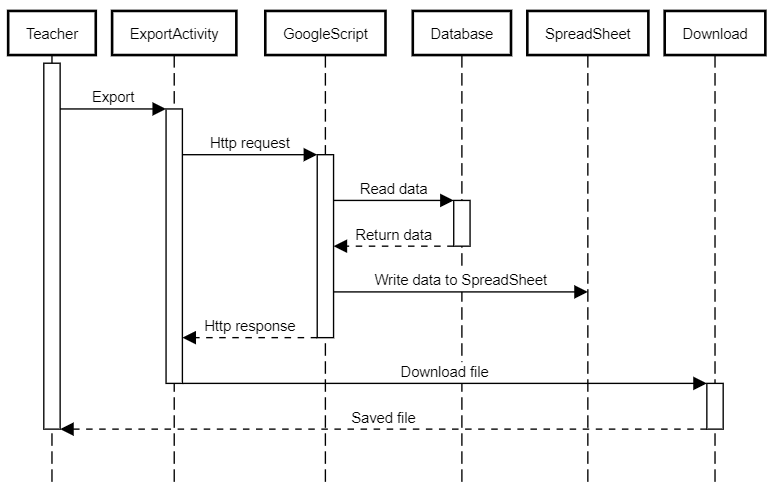
\includegraphics[width=350px]{seq_export.png}
	\caption{Jelenlétek exportálása a tanár által}
	\label{fig:seq2}
\end{figure}

\hfill \break
A ~\ref{fig:seq3} ábra bemutatja, ahogy a diák kiválasztja a tantárgyat, amiből szeretné megtekinteni a jelenléteit, majd lekérve a jelenléteket, láthatóvá válik egy listában, jelölve a pótlásokat is.\\

\begin{figure}[H]
	\centering
	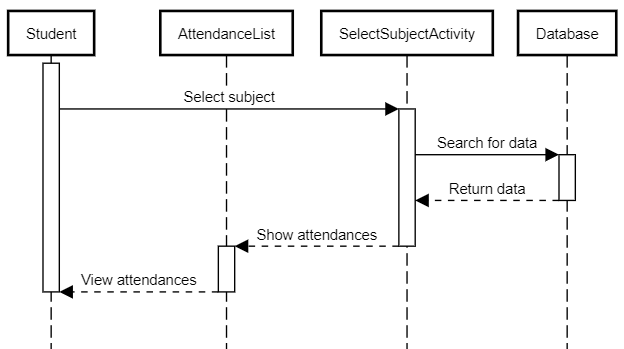
\includegraphics[width=350px]{seq_ViewAtt.png}
	\caption{Jelenlétek listázása a diák által}
	\label{fig:seq3}
\end{figure}

\hfill \break

\subsection{Fő modulok leírása}
\subsubsection{Diák alkalmazás fontosabb komponensei}
\begin{itemize}
	\item \textbf{Regisztráció}\\
	Az alkalmazás használatához szükség van regisztrációra, amely által a szükséges adatok tárolásra kerülnek az adatbázisban.
	A diák esetében ezek az adatok a szak, a teljes név, a Neptun azonosító, az e-mail cím, valamint egy jelszó. Kiegészítjük ezeket egy eszköz azonosítóval, ami segít abban, hogy amennyire lehet megakadályozzuk a visszaéléseket. Ez azt jelenti, hogy regisztrációkor a diákhoz rendelünk egy egyedi eszköz azonosítót, ami egy random generált karakterlánc összefűzve a diák Neptun kódjával, és regisztrációkor ezt is mentjük a diák személyes adatai mellett, így egy eszközről csak egy diák regisztrálhat és jelentkezhet az órára.\\
	Az adatbázisba való beszúrás úgy történik, hogy kiválasztjuk a Student JSON objektumot és abba mentjük az új diákot, kulcsként a NeptunId-ját használva.\\
	A műveletet az ~\ref{fig:diak_reg} ábrán látható kódrészlet szemlélteti. \\
		
	\begin{figure}[H]
		\centering
		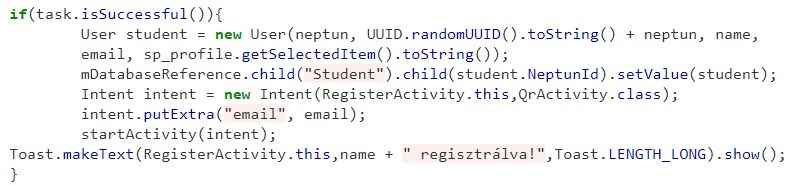
\includegraphics[width=400px]{student_reg2.jpg}
		\caption{Diák adatinak beszúrása az adatbázisba}
		\label{fig:diak_reg}
	\end{figure}

\hfill \break

	Egy Student JSON objektum a következőképpen épül fel:
	
	\begin{figure}[H]
		\centering
		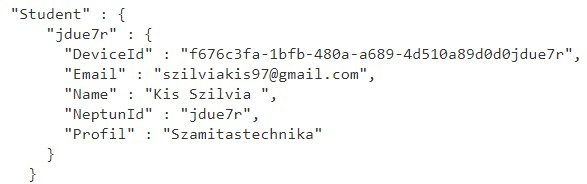
\includegraphics[width=360px]{student_json2.jpg}
		\caption{Diák JSON objektum az adatbázisban}
	\end{figure}

\newpage
	
	\item \textbf{QR kód generálás a diák adataival}\\
	A QR kód tartalmazza a diák szakját, nevét, Neptun azonosítóját, valamint az egyedi eszköz azonosítót. Az alkalmazásba való bejelentkezés során az e-mai alapján azonosítva lesz a diák az adatbázisban, és az sikeres belépést követően megjelenik egy üdvözlő szöveg.  Mivel a diák személyes adatai regisztráció során bekerültek az adatbázisba, így a QR kód generálásához lekérjük őket, és meghívva a \textit{TextToImageEncode(String Value)} függvényt, amely a QR kód formai előállításáért felel, paraméterként kapja a diák adatait JSON formátumban, ezzel előállítjuk az egyedi azonosítót a diák számára egy QR kód formájában.\\
	Az említett művelet kódrészlete az ~\ref{fig:create_qr} ábrán tekinthető meg.\\
	
	\begin{figure}[H]
		\centering
		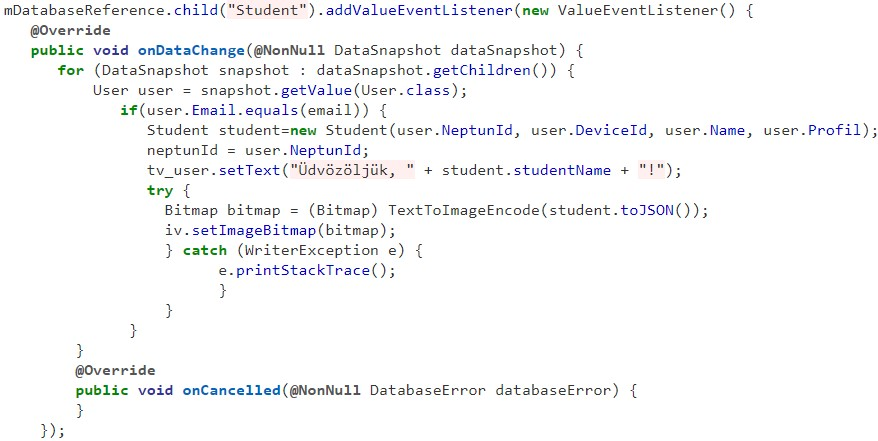
\includegraphics[width=400px]{qr_data2.jpg}
		\caption{QR kód létrehozása a diák személyes adataival}
		\label{fig:create_qr}
	\end{figure}

\newpage

A fent említett QR kód generáló függvény a következőképp néz ki:
	\begin{figure}[H]
		\centering
		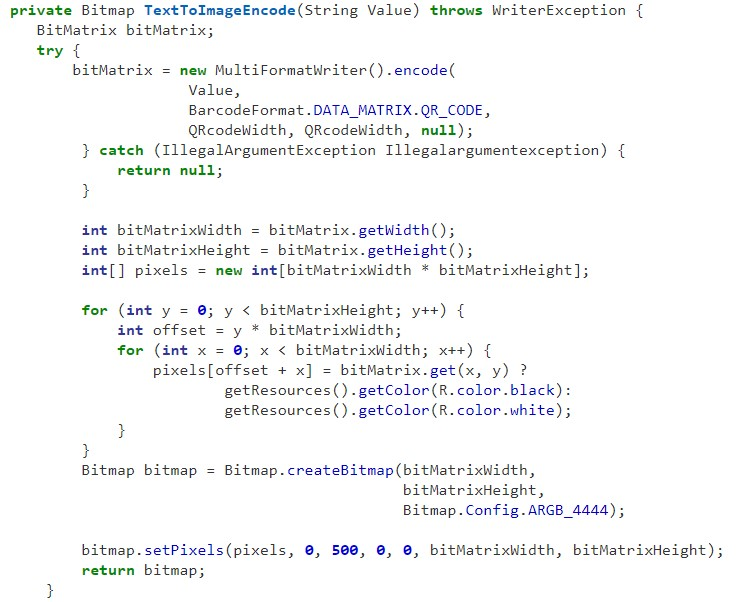
\includegraphics[width=380px]{qr.jpg}
		\caption{QR kód előállítása}
	\end{figure}


\hfill \break

	
\item \textbf{Jelenlétek megtekintése}\\
	A korábbi jelenlétek megtekintéséhez adott diák esetében végigiterálunk a jelenléti listán, és ahol a tárolt Neptun azonosító megegyezik a bejelentkezett diák Neptunjával, megjelenítjük jelenléteit egy Recyclerview listában. A jelenlétek jelölésére jelölőnégyzeteket használunk: ha a négyzet üres, arra az alkalomra nincs jelenlét, ha zöld, a jelenlét órarend szerinti időben volt, ha sárga színű, pótlás történt az adott órán. Ezeket a ~\ref{fig:view_attendance} kódrészlet alapján állítjuk be.\\

	\begin{figure}[H]
		\centering
		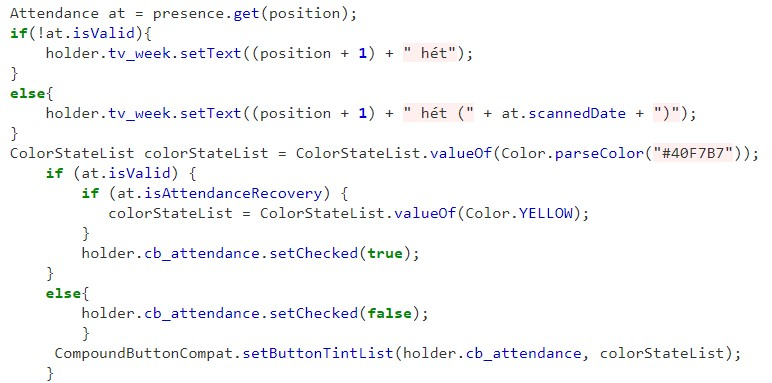
\includegraphics[width=400px]{view_att_stud.jpg}
		\caption{Jelenlétek jelölése}
		\label{fig:view_attendance}
	\end{figure}

\hfill \break


\subsubsection{Tanár alkalmazás fontosabb komponensei}

	\item \textbf{QR kód szkennelés}\\
	A diák alkalmazás által generált QR kód beolvasása a tanár alkalmazás feladata. Ez a művelet teszi lehetővé, hogy a diák adatai bekerüljenek az adatbázisba, ezzel jelezve a jelenlétét az adott órán.\\
	A tanár egy gomb segítségével tudja elindítani a szkennelést, amely által elindul a kamera, és a diák QR azonosítója fölé tartva, bármilyen irányból tudja értelmezni, így olvasva ki a kódolt adatokat. A programban a kamera elindításakor megadjuk, hogy milyen típusú kódot tudjon szkennelni és értelmezni, esetünkben a kódtípus a QR.\\
	
	\begin{figure}[H]
		\centering
		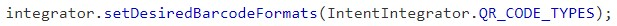
\includegraphics[width=360pt]{scan2.jpg}
		\caption{Szkennelhető típus beállítása QR kódra}
	\end{figure}

	Miután a kamera elindult, és beolvasásra került a diák azonosítója, lekérjük a beszkennelt QR kód tartalmát, amiről tudjuk, hogy egy JSON String. Első sorban ellenőrizzük, hogy a szkennelés sikeres volt-e, amennyiben igen, lekérjük a tartalmát. Ha a tartalma nem null, azaz van szkennelt adat, egy JSON objektumot csinálunk belőle. Amint létrejött az objektum, soronként olvassuk belőle a tagokat és létrehozunk egy Student objektumot. Ezt az objektumot fogjuk hozzáadni az adatbázisban a jelenléthez. A megadott adatok mellett tárolva lesz a szkennelés dátuma és időpontja is. A művelet sikerességét egy megerősítő üzenet jelzi. Ha a QR kód nem tartalmazza a szükséges adatokat, megjelenik a hibaüzenet.\\
	
	\begin{figure}[H]
		\centering
		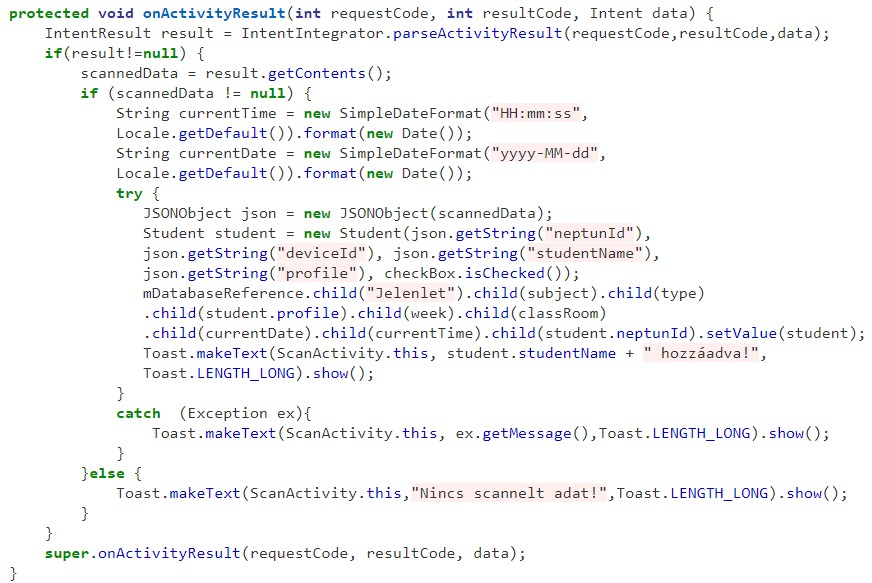
\includegraphics[width=400px]{teacher_scanStudent2.jpg}
		\caption{Adatok kiolvasása és mentése QR kódból}
	\end{figure}
	
\break

	\item \textbf{Diák manuális hozzáadása}\\
	Amennyiben a diák nem rendelkezik a megfelelő eszközzel az alkalmazás telepítésére, a tanárnak lehetősége van manuálisan hozzáadni az adatbázishoz. Ezáltal a tanár feladata a diák szakjának, nevének, valamint Neptun azonosítójának a megadása, illetve pótlás esetén, annak megjelölése. Ezek az adatok ugyanúgy mentve lesznek az adatbázisban, mint szkennelés esetén. Ebben az esetben is a tantárgyi adatok mellett tárolva lesz a beviteli dátum és idő is.\\
	Mindhárom adat megadása kötelező. Az eszköz azonosító helyett egy \enquote{From teacher} szöveg jelzi, hogy az adatok a tanár által lettek megadva.\\
	Az alábbi kódrészlet a manuális adatok mentését szemlélteti:\\
	
	\begin{figure}[H]
		\centering
		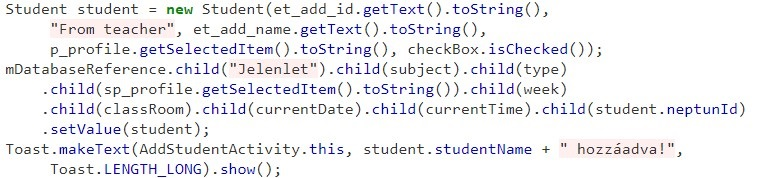
\includegraphics[width=380px]{manuallyAdd2.jpg}
		\caption{Diák jelenlétének manuális bevitele}
	\end{figure}

\hfill \break
	A két lehetséges módon történő jelenlét hozzáadásának folyamatát az ~\ref{fig:activity} ábrán látható aktivitás diagram szemlélteti.

	\begin{figure}[H]
		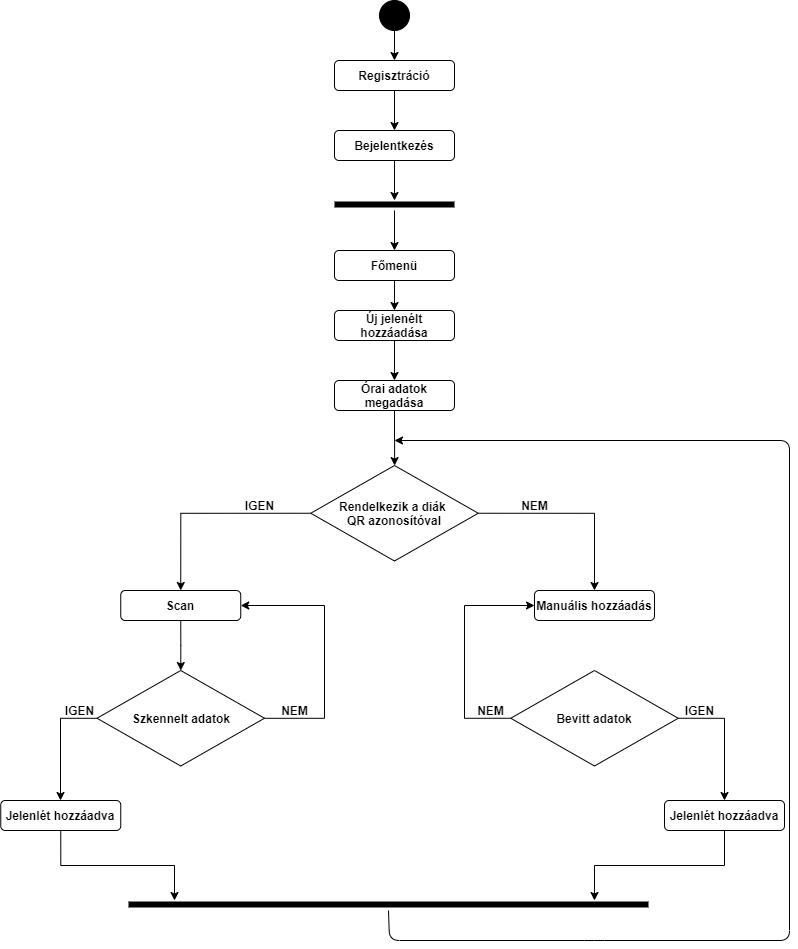
\includegraphics[width=\textwidth]{addAttActivity.png}
		\caption{Jelenlét hozzáadásának aktivitás diagramja}
		\label{fig:activity}
	\end{figure}

	
	\item \textbf{Adott diák jelenléteinek megjelenítése}\\
	A diák korábbi jelenléteinek megtekintésére a tanár alkalmazáson keresztül is lehetőség van. Ez szintén egy recyclerview listával van megvalósítva, ahol létrehozunk 14 elemet (mivel ideális esetben 14 hétből áll az oktatási időszak). A hét, a szkennelés dátuma és a jelenlét típusa (zöld - sárga jelölőnégyzet) jelenti a listaelemet.\\
	A jelenléti adatokat az adatbázisból kérjük le, majd a bejelentkezett diák adatait, valamint a jelenléteinek a számát megjelenítjük a listában.\\
	Az alábbi ábrán látható az adatbázisból való lekérdezés kódrészlete.	
	
	\begin{figure}[H]
		\centering
		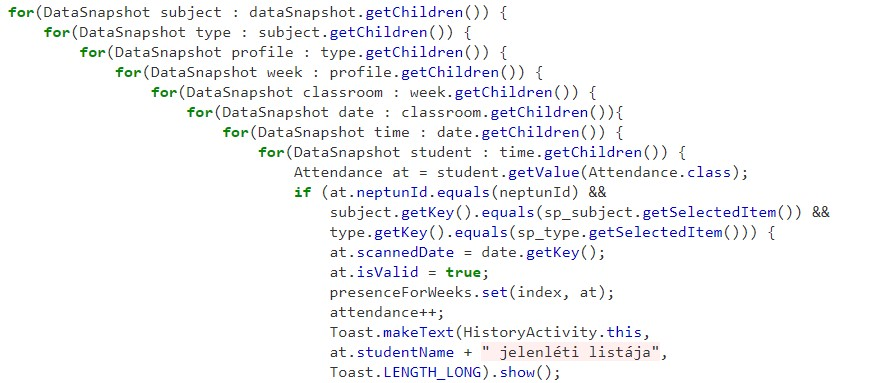
\includegraphics[width=400px]{attendances2.jpg}
		\caption{Jelenléti adatok lekérése az adatbázisból}
	\end{figure}


\newpage

	Az alábbi képen látható egy diák jelenlétének tárolási módja az adatbázisban:\\
	
	\begin{figure}[H]
		\centering
		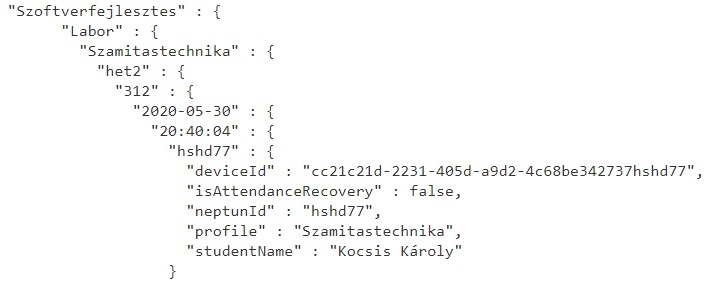
\includegraphics[width=380px]{fbAttendance2.jpg}
		\caption{Jelenlét JSON objektum az adatbázisban}
	\end{figure}
	
	\item \textbf{Jelenlétek exportálása}\\
	A Firebaseben lévő jelenléti adatok táblázatba való exportja Google Apps szkriptben került megvalósításra. \\
	A táblázatok létrehozásának főbb lépései a következők:
	 
	\begin{itemize}
		\item\textbf{Spreadsheet létrehozása}\\
		A Spreadsheeteket tárgy alapján hozzuk létre, megkülönböztetve a tárgy típusa szerint (előadás - labor), végigiterálva a jelenléti struktúrán. A tantárgyon belül külön munkalapokat hozunk létre szakonként.\\
		Az adatok átláthatósága miatt, valamint a jelenlétek egyszerűbb követése érdekében a jelenlétek szakokon belül külön táblázatban jelennek meg. Ezt a Munkalapok duplikálásával oldjuk meg, valamint elnevezzük a szakok szerint.
		Ennek a Javascriptben való megvalósítás a ~\ref{fig:spreadsheet} ábrán látható.\\
		
		\begin{figure}[H]
			\centering
			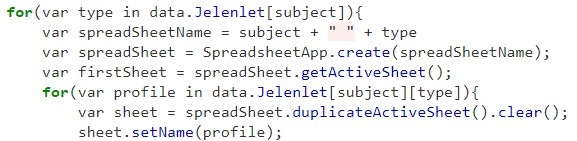
\includegraphics[width=300px]{create_sheet2.jpg}
			\caption{Spreadsheet létrehozása}
			\label{fig:spreadsheet}
		\end{figure}
	
\hfill \break

	\item\textbf{Adatok beszúrása a táblázatba}\\
	Végigmenve a jelenléti listán, ellenőrizzük, hogy az adott diák szerepel-e már a táblázatban vagy sem.\\
	Amennyiben a diák korábban már hozzá lett adva a táblázathoz, csak az újabb jelenlétet szúrjuk be, ami lehet akár pótlás is. Tehát, ahogy az alábbi kódrészletben látható, új diák esetén beszúrjuk magát a diák struktúrát, valamint a hozzá tartozó jelenlétet/pótlást, míg ellenkező esetben csak egy újabb jelenlétet adunk hozzá a már létező diákhoz.\\
	A getNumberFromWeekIndicator(week) függvény segítségével kapjuk meg a hét számát, azaz, hogy pontosan hányadik hétre kell beszúrni a jelenlétet.
	Emellett a diák jelenlétét az időpont jelzi, míg a pótlást a teljes dátum és idő, így könnyen követhető mikor történt és melyik pótlás.\\
	A táblázat tartalmaz egy sorszámot, a diák nevét, Neptun azonosítóját és a jelenléteit 14 hétre.\\ 
	A sorok végén egy számláló segítségével számoljuk diákonként a jelenlétek számát.\\
	
	
	\begin{figure}[H]
		\centering
		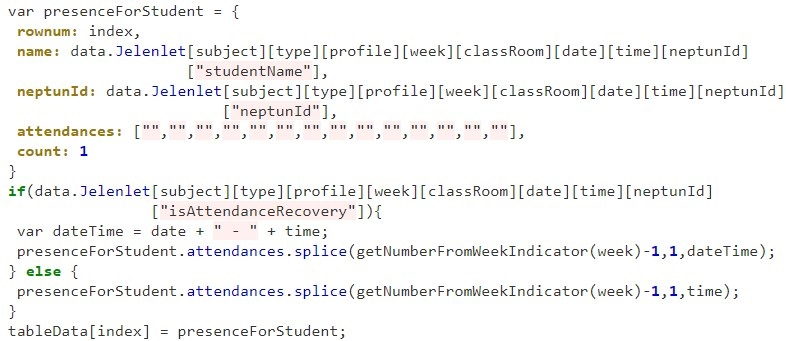
\includegraphics[width=380px]{addToTable3.jpg}
		\caption{Új diák beszúrása a táblázatba}
	\end{figure}

	Végigmegyünk a jelenléteken (tantárgy, típus, szak), és adjuk hozzá a táblázathoz:\\

	\begin{figure}[H]
		\centering
		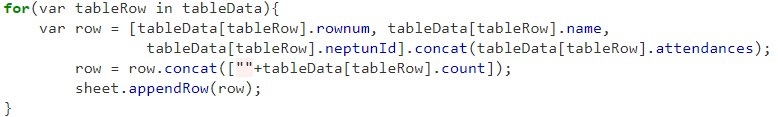
\includegraphics[width=380px]{addToTable4.jpg}
		\caption{Jelenlétek hozzáadása a táblázathoz}
	\end{figure}

\hfill \break

	
	\end{itemize}
	
	\item \textbf{Jelenlétek letöltése}\\
	A tanár alkalmazás lehetővé teszi a jelenléti táblázatok letöltését három formátumban: xlsx, pdf, csv.\\ A letöltött fájlok lokálisan tárolva lesznek, illetve minden letöltéskor két fájl töltődik egyszerre: az adott tantárgy előadás és labor jelenléti táblázatai, amennyiben ezek léteznek.
	A letöltés szintén a szkripten keresztül történik, mivel a létrehozott táblázat letöltési linkjét érjük el az alkalmazásban.\\
	Az alkalmazás a Google Apps szkript URL linkjén keresztül kommunikál a szkripttel. A szkript oldalon bevezetjük internetes alkalmazásként, majd a kapott URL-en keresztül érjük el az Android alkalmazásban.\\

	A szkriptben tehát megkapjuk a jelenléti táblázat letöltéséhez szükséges linket:\\
	
	\begin{figure}[H]
		\centering
		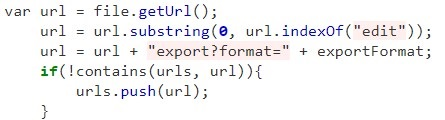
\includegraphics[width=250px]{script_link2.jpg}
		\caption{Google Apps szkript táblázat letöltési link létrehozása}
	\end{figure}

	A tanár feladata az alkalmazásban kiválasztani a letölteni kívánt tantárgyhoz tartozó jelenléti listát, valamint a formátumot. Amennyiben nem választ formátumot, automatikusan xlsx-ben lesz letöltve a fájl.
	
\hfill \break
	
	\item \textbf{Belépés a Google tanterembe}\\
	Minden tanár rendelkezik saját tantárgyakkal, amelyekhez tartozik egy-egy Google tanterem link, ezzel is hozzájárulva az oktatás hatékonyabbá tételéhez.\\
	A linkek az adatbázisban vannak tárolva, a tanár adatai mellett. Egyik listában vannak megadva a tantárgyak, egy másik listában pedig a hozzá tartozó linket. A pozíciókat társítjuk egymáshoz, így rendelve a linket az adott tárgyhoz.\\
	Az adatbázisban tárolt tanár objektum a két listával:\\
	
	
	\begin{figure}[H]
		\centering
		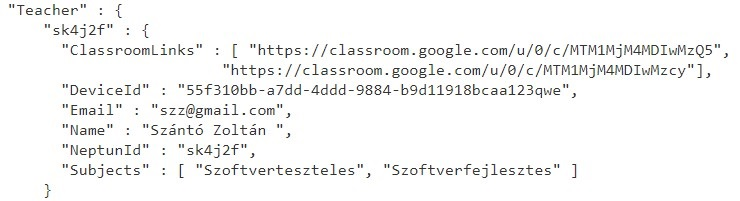
\includegraphics[width=380px]{teacherDB2.jpg}
		\caption{Tanár JSON objektum az adatbázisban}
	\end{figure}
	
	Amennyiben a tantárgyhoz van rendelve Google tanterem, megnyitható az alkalmazáson keresztül. A megnyitáshoz egy böngészőre van szükség, amelyet legelső futtatásnál választunk, amennyiben több lehetőséget kínál az eszköz.\\
	
	\begin{figure}[H]
		\centering
		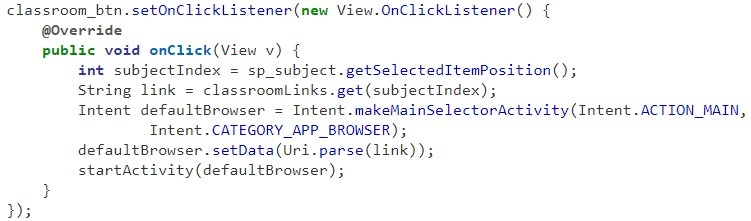
\includegraphics[width=380px]{classroomT2.jpg}
		\caption{Google tanterem megnyitása}
	\end{figure}


\hfill \break


	\item \textbf{Naptáresemény létrehozása}\\
	A tanár alkalmazás lehetőséget kínál naptáresemény létrehozására, különböző tantárgyi adatok megadásával. Ezek az adatok az esemény címe, leírása, kezdete valamint a vége (ami az időpontot illeti), illetve az esemény dátuma. Az adatok megadása után megnyílik a Google naptár, ahova be lesznek szúrva a tanár által megadott információk, valamint csatolható még például Google meet link is, amennyiben igény van rá. Mindemellett ami a címzettet illeti megadhat tetszőleges címet, illetve választhat a különböző Google tantermek közül. Amennyiben kiválaszt egy tantermet, a benne lévő diákok e-mailt kapnak az eseményről, valamint bekerül a saját naptárukba is, illetve emlékeztetőt is fognak kapni az eseményről.\\

	\begin{figure}[H]
		\centering
		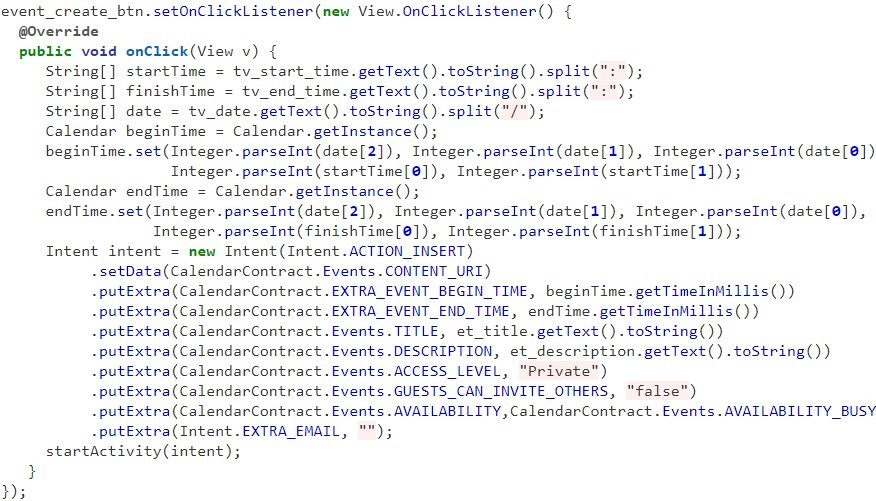
\includegraphics[width=400px]{calendar.jpg}
		\caption{Naptáresemény létrehozása}
	\end{figure}

\hfill \break


	\item \textbf{Csoportos e-mail küldése}\\
	Hasonlóan a naptáresemény létrehozásához, az e-mail küldés esetén is szükséges megadni néhány adatot. Ide tartozik a szak és a tantárgy kiválasztása, a tárgy, valamint az üzenet, ezek mellett lehetőség van különböző típusú állományok csatolására is. Az e-mail címzettjei a szak és tantárgy alapján kerülnek megjelölésre: adott tárgyhoz tartozó egy szakon belüli diákok fogják megkapni az üzenetet.\\
	Ahogy az eseménynél is volt, itt is szükség van egy e-mail küldő alkalmazás meglétére az eszközön, majd kiválasztva azt a tanár által megadott információk beillesztésre kerülnek. Itt még tetszőlegesen módosíthatóak az adatok. Ezután csak a megszokott módon elküldjük az e-mailt.\\
	Az adatok beszúrását az ~\ref{fig:spreadsheet} ábrán lévő kódrészlet szemlélteti.

	\begin{figure}[H]
		\centering
		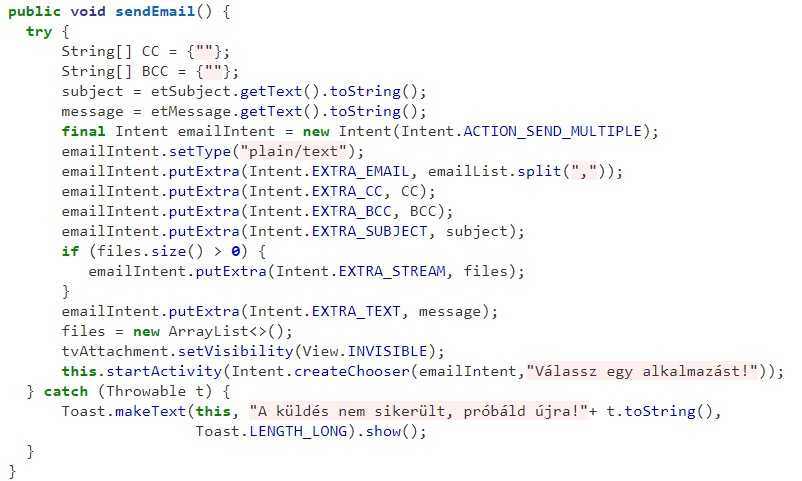
\includegraphics[width=400px]{send_mail.jpg}
		\caption{E-mail küldése a diákoknak}
		\label{fig:send_mail}
	\end{figure}
	
\end{itemize}

\hfill \break
Az említett modulok mellett még vannak más szükséges komponensek, amik szintén hozzájárulnak a rendszer egészéhez.


\newpage

\section{Használt technológiák}
A projekt kivitelezése során a következő technológiák kerültek felhasználásra:

\subsection{Android Studio}
Az Android Studio az IntelliJ IDEA alapú hivatalos integrált fejlesztői környezet (IDE) az Android alkalmazásfejlesztéshez. Az IntelliJ hatalmas kódszerkesztője és fejlesztőeszköze mellett az Android Studio több olyan funkcionalitással rendelkezik, amelyek növelik a hatékonyságot az Android-alkalmazások fejlesztésekor. Ilyen például a rugalmas Gradle-alapú build rendszer, a gyors és funkciókban gazdag emulátor, az egységes környezet, ahol lehetőség van az összes Android-eszköz fejlesztésére, stb \cite{9}.\\
A jelenlétkezelő alkalmazásunk egy mobil applikáció, ezért Android operációs rendszerre terveztük. Android Studio-ban, Java nyelvben történt a fejlesztés. A projekt során két külön Android alkalmazást hoztunk létre: egyet a tanár részére (Teacher App), egyet pedig a diák részére (Student App). Azért választottuk ezt a technológiát, mivel a célfelhasználók legtöbbje Andoid operációs rendszert támogató okostelefonnal rendelkezik.

\subsection{Google Apps Script}
A Google Apps Script egy gyors alkalmazásfejlesztő platform, amely egyszerűvé teszi a G Suite (programcsomag, amely a Google által kínált különböző felhő alapú szoftverekből áll) alkalmazásba integrált alkalmazások létrehozását. A kódírás JavaScript-ben történik, valamint hozzáférést biztosít a beépített könyvtárakhoz a G Suite alkalmazások eléréséhez, mint például a Gmail, a Naptár, a Drive és így tovább. Nem kell semmit telepíteni - közvetlenül a böngészőnkben létrehozunk egy kódszerkesztőt, és a szkriptek a Google szerverein futnak \cite{10}.\\
A dolgozatban fontos szerepe volt a Google Apps Script alkalmazásfejlesztő platformnak, mivel így lehetőségünk volt az általunk létrehozott Android alkalmazásból elérni az olyan felhőalapú alkalmazásokat, mint a Drive, amit arra használunk, hogy biztosítsuk a tanár számára a jelenlétek exportálását egy Google táblázatba.

\subsection{Firebase}
A Firebase egy backend-as-a-service (Baas). A fejlesztők számára különféle eszközöket és szolgáltatásokat nyújt, amelyek segítenek minőségi alkalmazások fejlesztésében. A Google infrastruktúrájára épül.\\
A Firebase a NoSQL felhő alapú adatbázisok közé tartozik, amely az adatokat JSON-szerű dokumentumokban tárolja \cite{11}. \\
A projekt megvalósítása során a Firebase két fő funkcióját vettük igénybe:

\begin{itemize}
	\item \textbf{Valós idejű adatbázis}\\
	Az adatokat valós időben szinkronizálja az összes kliens között, és elérhetővé válik, amikor az alkalmazás offline állapotba kerül \cite{12}. \\
	Az általunk fejlesztett alkalmazásnál ez a funkcionalitás elengedhetetlen volt, mivel több felhasználóról van szó, valamint az adatok mindig naprakészek és elérhetőek kell legyenek az alkalmazást igénybe vevők számára.\\
	
	\item \textbf{Hitelesítés}\\
	A legtöbb alkalmazásnak tudnia kell a felhasználó személyazonosságát. A felhasználó személyazonosságának ismerete teszi lehetővé az alkalmazás számára, hogy biztonságosan mentse a felhasználói adatokat a felhőben, és ugyanazt a személyre szabott élményt biztosítsa a felhasználó összes eszközén.\\
	A Firebase hitelesítés háttér-szolgáltatásokat, könnyen használható SDK-kat és kész felhasználói felület-könyvtárakat biztosít a felhasználók hitelesítésére az alkalmazásokhoz. Támogatja a hitelesítést jelszavak, telefonszámok, különböző alkalmazások, például Google, Facebook, és még sok más használatával \cite{13}.\\
	A jelenlétkezelő alkalmazásunkban az e-mail - jelszó párost választottuk a felhasználók azonosítására az adatbázisban, teljesen kihasználva a Firebase nyújtotta hitelesítési lehetőséget.
\end{itemize}

\subsection{GitHub}
A GitHub egy projekt menedzsment és egy kódverzió követő rendszer, amelyet a fejlesztők számára hoztak létre. Lehetővé teszi, hogy együtt dolgozzunk más emberekkel a világ minden tájáról, megtervezzük projektjeinket és nyomon kövessük a munkát \cite{14}.\\
A projekt fejlesztése során GitHub verziókövető rendszert használtunk a munkafolyamat követésére, illetve a feladatok menedzselésére is, kihasználva a GitHub ezen funkcióját is.

\subsection{LaTeX}
A LaTeX egy dokumentum-előkészítő rendszer. Az felhasználó jelölő címkézési konvenciókat (tag) használ a dokumentum általános szerkezetének meghatározására (típus), a szöveg egészének stilizálására (betűstílus), idézetek és hivatkozások hozzáadására, stb \cite{15}.\\
A teljes dokumentum megírására a LaTeX szövegformázó rendszerben történt.

\hfill \break




\section{A felhasználói felület bemutatása}
\subsection{Diák alkalmazás}
A diák alkalmazás elindításakor regisztrációra van szükség, amennyiben még nem regisztrált korábban. Ezt követően a rendszer küld egy üzenetet a megadott e-mail címre, amit kötelező visszaigazolni. Amíg ez nem történik meg, nem lehetséges a bejelentkezés. Amennyiben nem sikerül a visszaigazolás, lehetőség van újabb visszaigazoló e-mail küldésére. Az esetben, ha korábban már megtörtént a regisztrálás és visszaigazolás, a bejelentkezés lehetőséget kell válassza. Ha a bejelentkezés sikeres, egy újabb oldal kerül megjelenítésre, ahol a megadott adatokkal létrejön a QR azonosító (~\ref{fig:s_1} ábra).\\

	\begin{figure}[H]
		\centering
		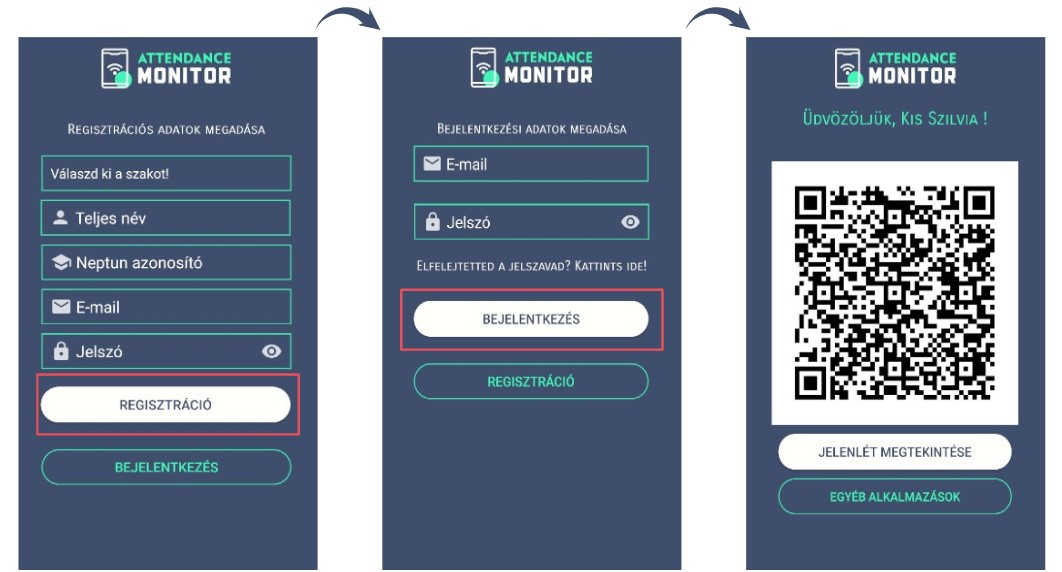
\includegraphics[width=380px]{s_1.jpg}
		\caption{Regisztráció és belépés a diák alkalmazásba}
		\label{fig:s_1}
	\end{figure}

\hfill \break
A főoldalon lehetőség van a korábbi jelenlétek megtekintésére is a tantárgy kiválasztásával. Itt megjelenítésre kerül a jelenlétek száma, illetve annak típusa is, amennyiben pótlás történt (~\ref{fig:s_2} ábra).

	\begin{figure}[H]
	\centering
	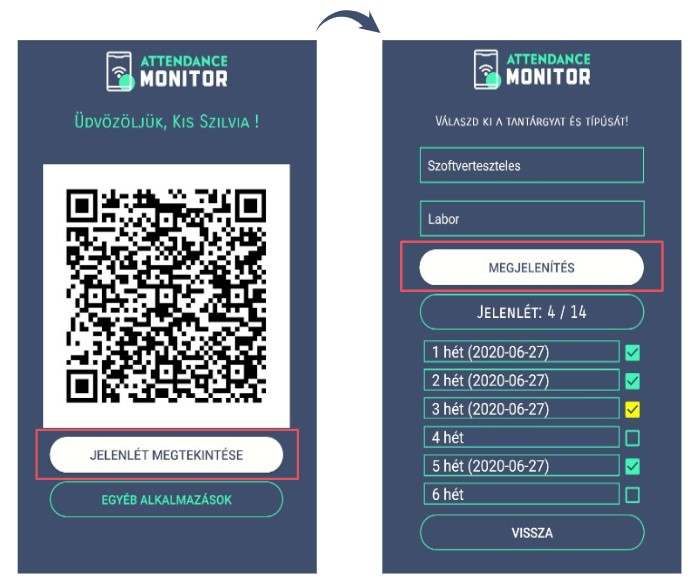
\includegraphics[width=280px]{s_2.jpg}
	\caption{Korábbi jelenlétek megtekintése}
	\label{fig:s_2}
\end{figure}

\hfill \break
Ugyanitt választható az \enquote{Egyéb alkalmazások} lehetőség, ezzel lehetősége nyílik a diáknak e-mail küldésre, ahol bármelyik tanárnak tud üzenetet küldeni csupán annak nevét ismerve, de ugyanakkor beléphet a Google tanterembe vagy akár a Neptun rendszerbe (~\ref{fig:s_3} ábra).

\begin{figure}[H]
	\centering
	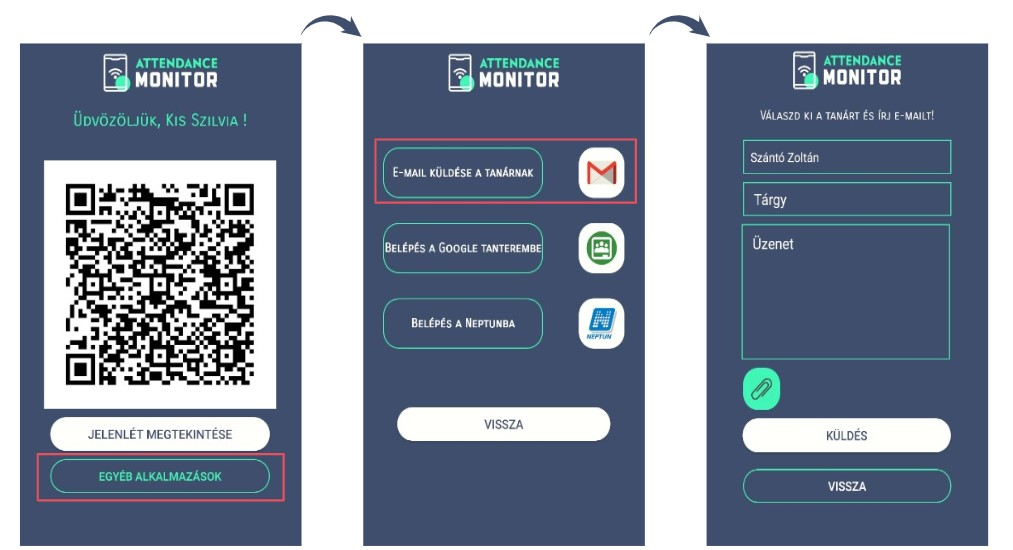
\includegraphics[width=380px]{s_3.jpg}
	\caption{E-mail küldés és egyéb alkalmazások}
	\label{fig:s_3}
\end{figure}

\hfill \break


\subsection{Tanár alkalmazás}
	A tanár alkalmazásban, hasonlóan a diákhoz van egy regisztrációs és egy bejelentkezési lehetőség, majd egy Menüsor fogadja a felhasználót (~\ref{fig:t_1} ábra).\\

\begin{figure}[H]
	\centering
	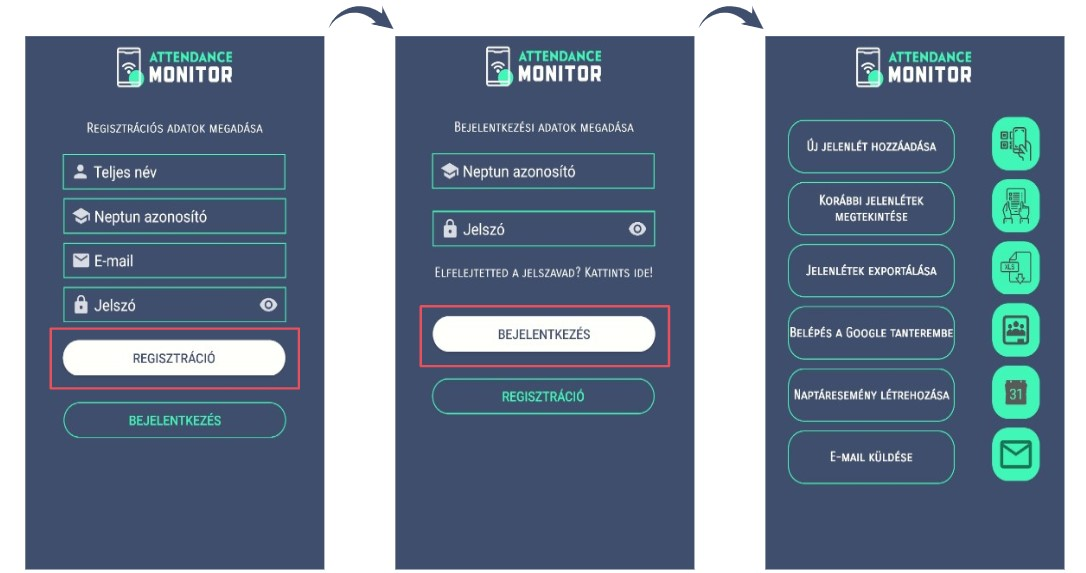
\includegraphics[width=380px]{t_1.jpg}
	\caption{Regisztráció és belépés a tanáralkalmazásban}
	\label{fig:t_1}
\end{figure}

\begin{itemize}
	\item {Új jelenlét hozzáadása}\\
	A új jelenlét hozzáadása menüpontot választva történik a jelenlét bevitele. Elsősorban a tantárggyal kapcsolatos adatokat kell megadni, majd két opció van a jelenlét bevitelér: szkennelt formában, vagy pedig manuálisa, amennyiben a diák nem rendelkezik az azonosítóshoz szükséges eszközzel. Ha a szkennelés lesz kiválasztva elindul a kamera, míg manuális hozzáadás esetében egy új ablak jelenik meg, ahol a szükséges adatokat kell megadni (~\ref{fig:t_2} ábra).
\end{itemize}


\begin{figure}[H]
	\centering
	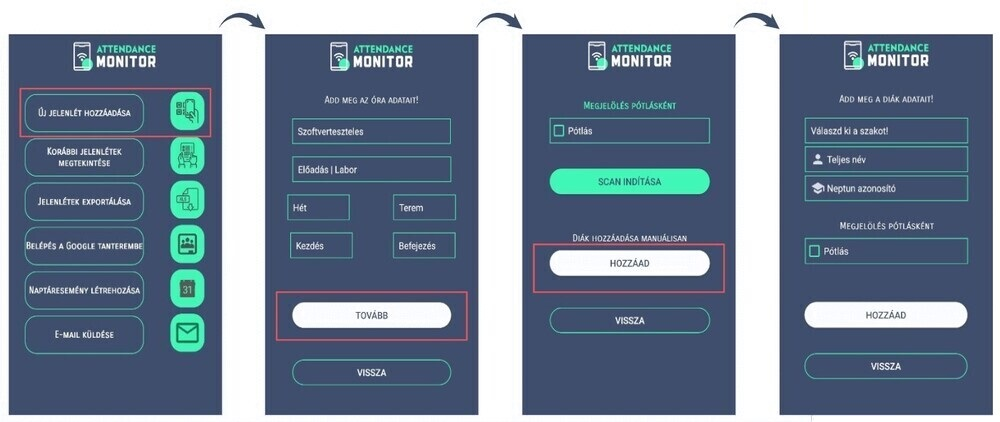
\includegraphics[width=480px]{t_2.jpg}
	\caption{Új jelenlét hozzáadása}
	\label{fig:t_2}
\end{figure}


\begin{itemize}
	\item {Korábbi jelenlétek megtekintése}\\
	A második opciót választva a tanárnak lehetősége van a diákok jelenléteinek megtekintésére, szak és tantárgy alapján. Ezt követően diákonként meg tudja nézni a részletes jelenléti adatokat (~\ref{fig:t_3} ábra).
\end{itemize}


\begin{figure}[H]
	\centering
	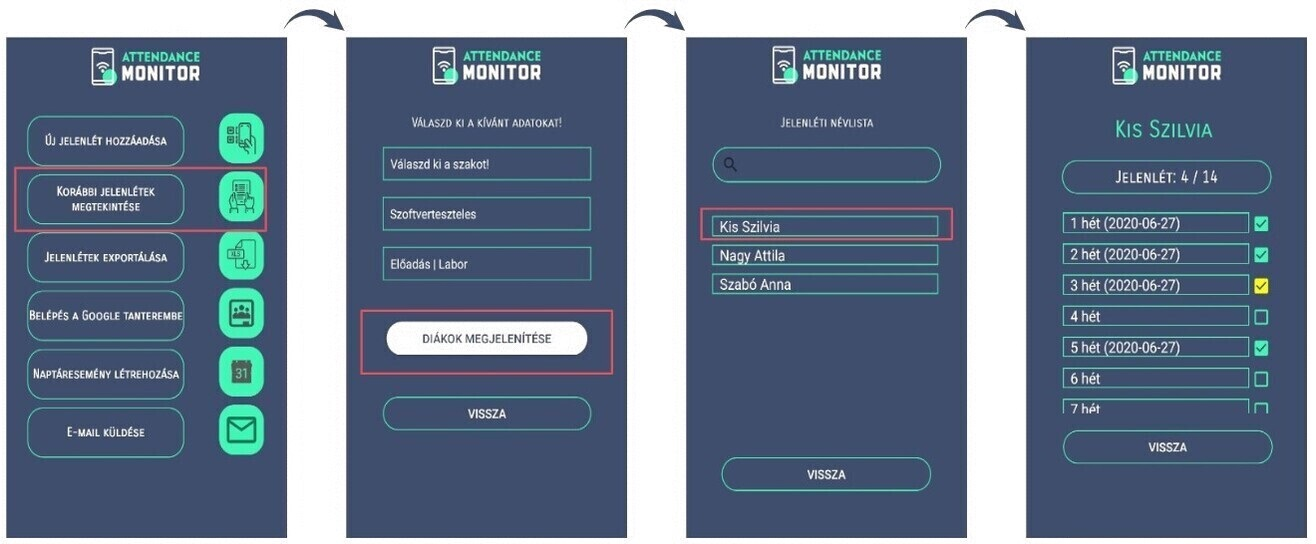
\includegraphics[width=480px]{t_3.jpg}
	\caption{Korábbi jelenlétek megtekintése}
	\label{fig:t_3}
\end{figure}


\begin{itemize}
	\item {Jelenlétek exportálása}\\
	A tanárnak lehetősége van a jelenléti táblázatok letöltésére tantárgyanként, valamint opcionálisan megadhatja a letölteni kívánt fájl formátumát is (~\ref{fig:t_4} ábra).
\end{itemize}


\begin{figure}[H]
	\centering
	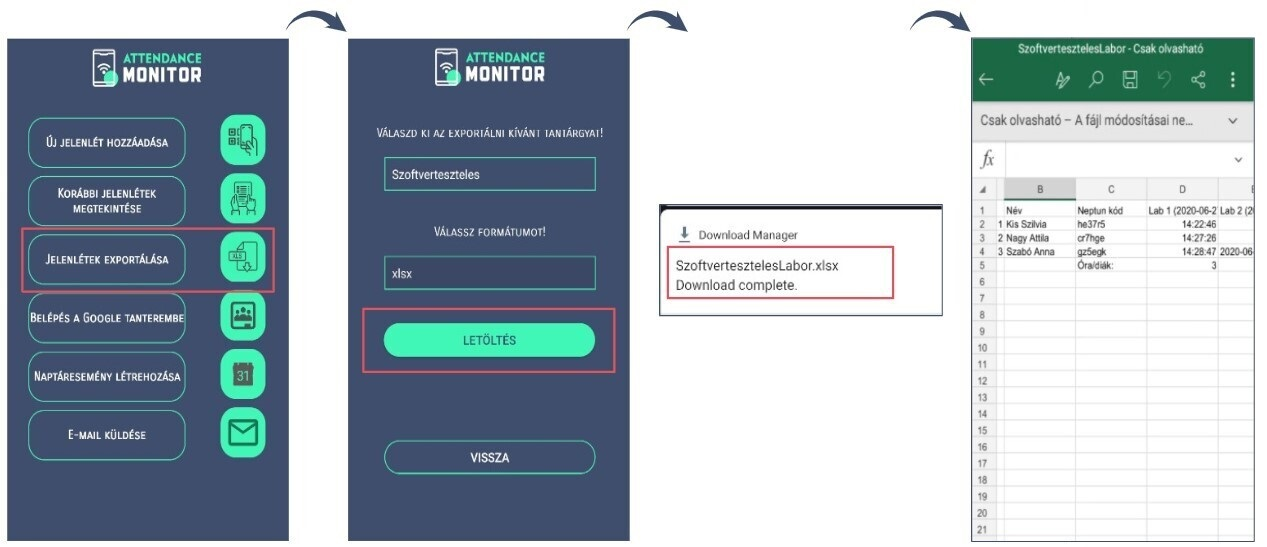
\includegraphics[width=480px]{t_4.jpg}
	\caption{Jelenlétek exportálása}
	\label{fig:t_4}
\end{figure}


\begin{itemize}
	\item {Belépés a Google tanterembe}\\
	Az alkalmazás következő menüpontja lehetővé teszi a Google tanterembe való belépést, kiválasztva a kívánt tantárgyat (~\ref{fig:t_5} ábra). 
\end{itemize}


\begin{figure}[H]
	\centering
	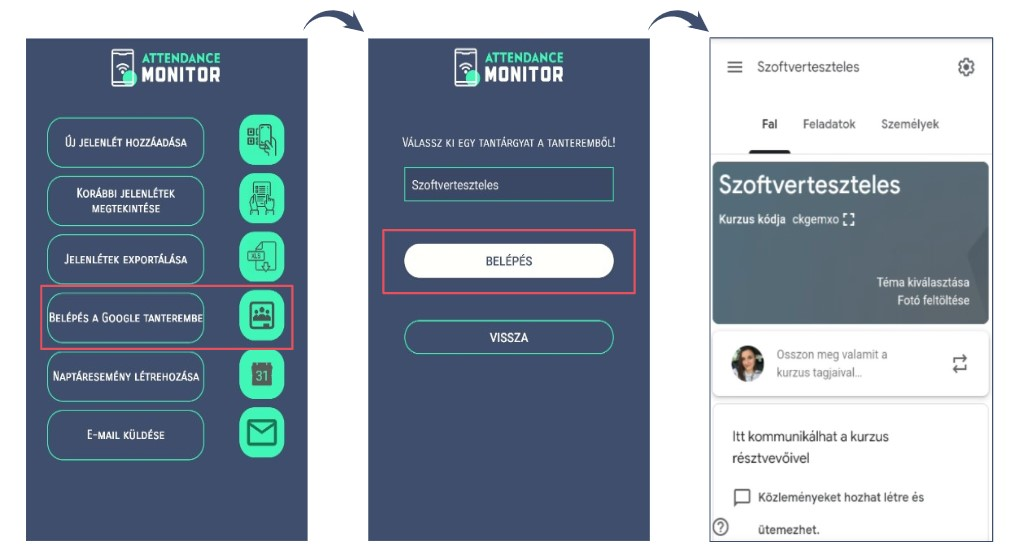
\includegraphics[width=380px]{t_5.jpg}
	\caption{Belépés a Google tanterembe}
	\label{fig:t_5}
\end{figure}


\begin{itemize}
	\item {Naptáresemény létrehozása}\\
	A tanár létrehozhat különböző eseményeket, ehhez szükséges megadnia az eseménnyel kapcsolatos információkat, majd ezek bekerülnek a Google naptár alkalmazásba, ahol lehetősége van elküldeni a diákoknak (~\ref{fig:t_6} ábra). 
\end{itemize}


\begin{figure}[H]
	\centering
	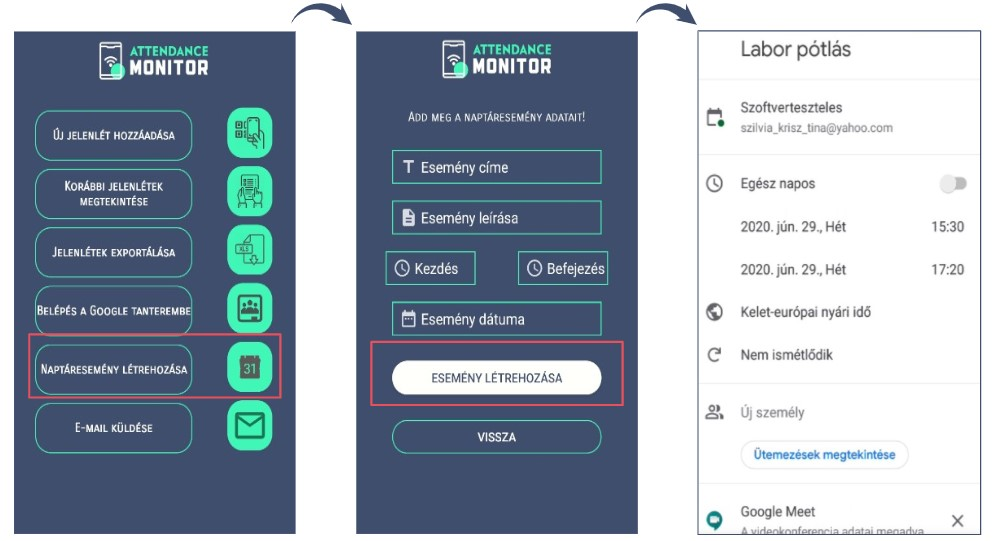
\includegraphics[width=380px]{t_6.jpg}
	\caption{Naptáresemény létrehozása}
	\label{fig:t_6}
\end{figure}

\begin{itemize}
	\item {E-mail küldése}\\
	Az e-mail küldés opció lehetővé teszi, hogy a tanár csoportos üzeneteket küldjön egy adott szaknak adott tantárggyal kapcsolatban. A szükséges információk kitöltése után kiválaszt egy e-mail küldő alkalmazás, ahova bekerülnek a megadott adatok, így továbbítható az e-mal tartalma. Emellett kiegészíthető egyéb információkkal, például Google meet link csatolása (~\ref{fig:t_7} ábra). 
\end{itemize}


\begin{figure}[H]
	\centering
	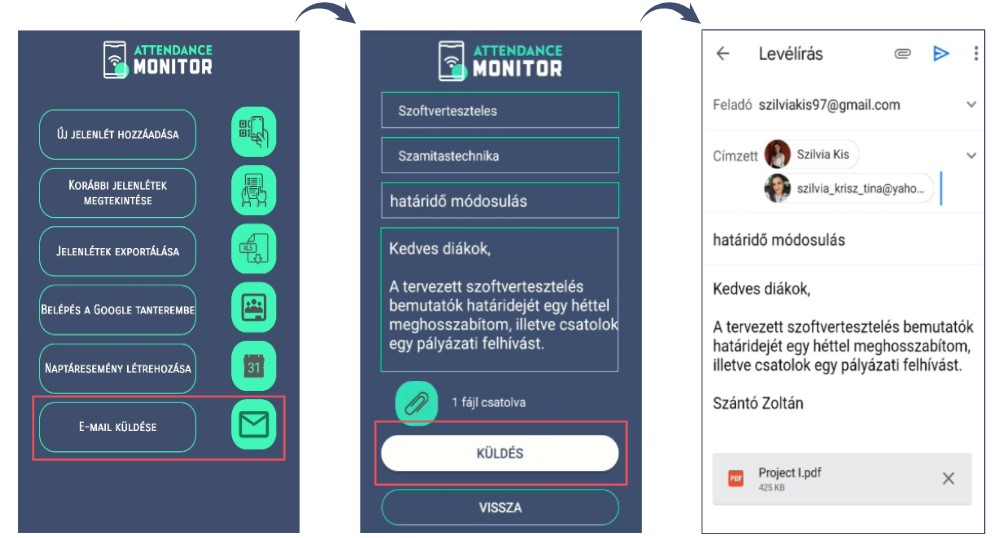
\includegraphics[width=380px]{t_7.jpg}
	\caption{E-mail küldése a diákoknak}
	\label{fig:t_7}
\end{figure}

\newpage


\section{Összefoglaló}
A projekten belül egy olyan szoftverrendszer megvalósítására került sor, amely hozzájárul az órákon való jelenlétkezelés megkönnyítéséhez, szem előtt tartva elsősorban a megbízhatóságot és hatékonyságot, valamint a könnyen kezelhetőséget tanárok és diákok számára egyaránt. 
Az alkalmazás lehetőséget nyúlt a diák számára, hogy saját okostelefonja segítségével igazolja jelenlétét az adott órán, illetve, hogy korábbi jelenléteit követni tudja. Emellett lehetősége van e-mail küldésére a tanárnak, ahol a címzett megadásához csupán a tanár nevének a kiválasztására van szükség egy listából. Ehhez hasonlóan a tanár alkalmazás lehetővé teszi a diákok azonosítását, kezelését, valamint kimentését néhány kattintással. A jelenlétkezelésen kívül lehetősége van naptár esemény létrehozására, illetve csoportos e-mail küldésére, kiválasztva a kívánt tantárgyat és szakot, akikhez címezni szeretné az üzenetet. \\
Elmondhatjuk, hogy érdemes kihasználni a technológia nyújtotta lehetőségeket, főleg amikor több felhasználót érintő alkalmazás fejlesztéséről van szó. Ezzel a korlátok minimálisra szűkíthetőek.\\
A legjobb mód az egyszerűség és a könnyen kezelhetőség, mivel az alkalmazás fő feladata a jelenlétkezelés, mint procedúra leegyszerűsítése. \\
Összességében sikerült megvalósítani egy működő és használatra kész rendszert, amely eleget tesz egy korszerű jelenlétkezelő alkalmazás elvárásainak.

\newpage

\section{Továbbfejlesztési lehetőségek}
Továbbfejlesztési lehetőségeink között a legfontosabb, hogy platformfüggetlenné tegyük az alkalmazást, így biztosítva minden felhasználó számára a biztos elérést.\\
Továbbá a jelenlegi rendszerünkben az Admin szerepkörű felhasználó számára nincs biztosítva külön felhasználói felület, így a közeljövőben szeretnénk ezt is megvalósítani.\\
A diák számára hasznos funkció lenne, ha az alkalmazás értesítést küldene a hamarosan kezdődő óráról.\\
Emellett megjelenítés, valamint könnyen kezelhetőség szempontjából kedvező ha a felhasználók rendelkeznek saját profillal az alkalmazáson belül, ahol különböző adatok módosítására lenne lehetőség a fiókjukkal kapcsoltban.\\
Végül de nem utolsó sorban szeretnénk, ha a felhasználónak lenne lehetősége személyre szabni az alkalmazást, különböző megjelenítési beállítások módosításával.

\newpage

\bibliographystyle{unsrt}
\bibliography{bibliography}


\newpage

\end{document}